In this section we document the Higgs search results in individual final states for the cut-based analysis.  

\subsection{Cut-based Analysis}

Figure~\ref{fig:uls_cut_0j}-\ref{fig:uls_cut_2j} show the expected and observed limits in the cut-based analysis 
for all contributing final states with the numbers tablulated in Table~\ref{tab:cutbase_uls_0jof}-\ref{tab:cutbase_uls_2j}. 

%%%%%%%%%%%%%%%%%%%%%%%%%%%%%%
\begin{figure}[!hbtp]
\centering
\subfigure[cut-based 0-Jet OF]{
\centering
\label{subfig:0jof_cut}
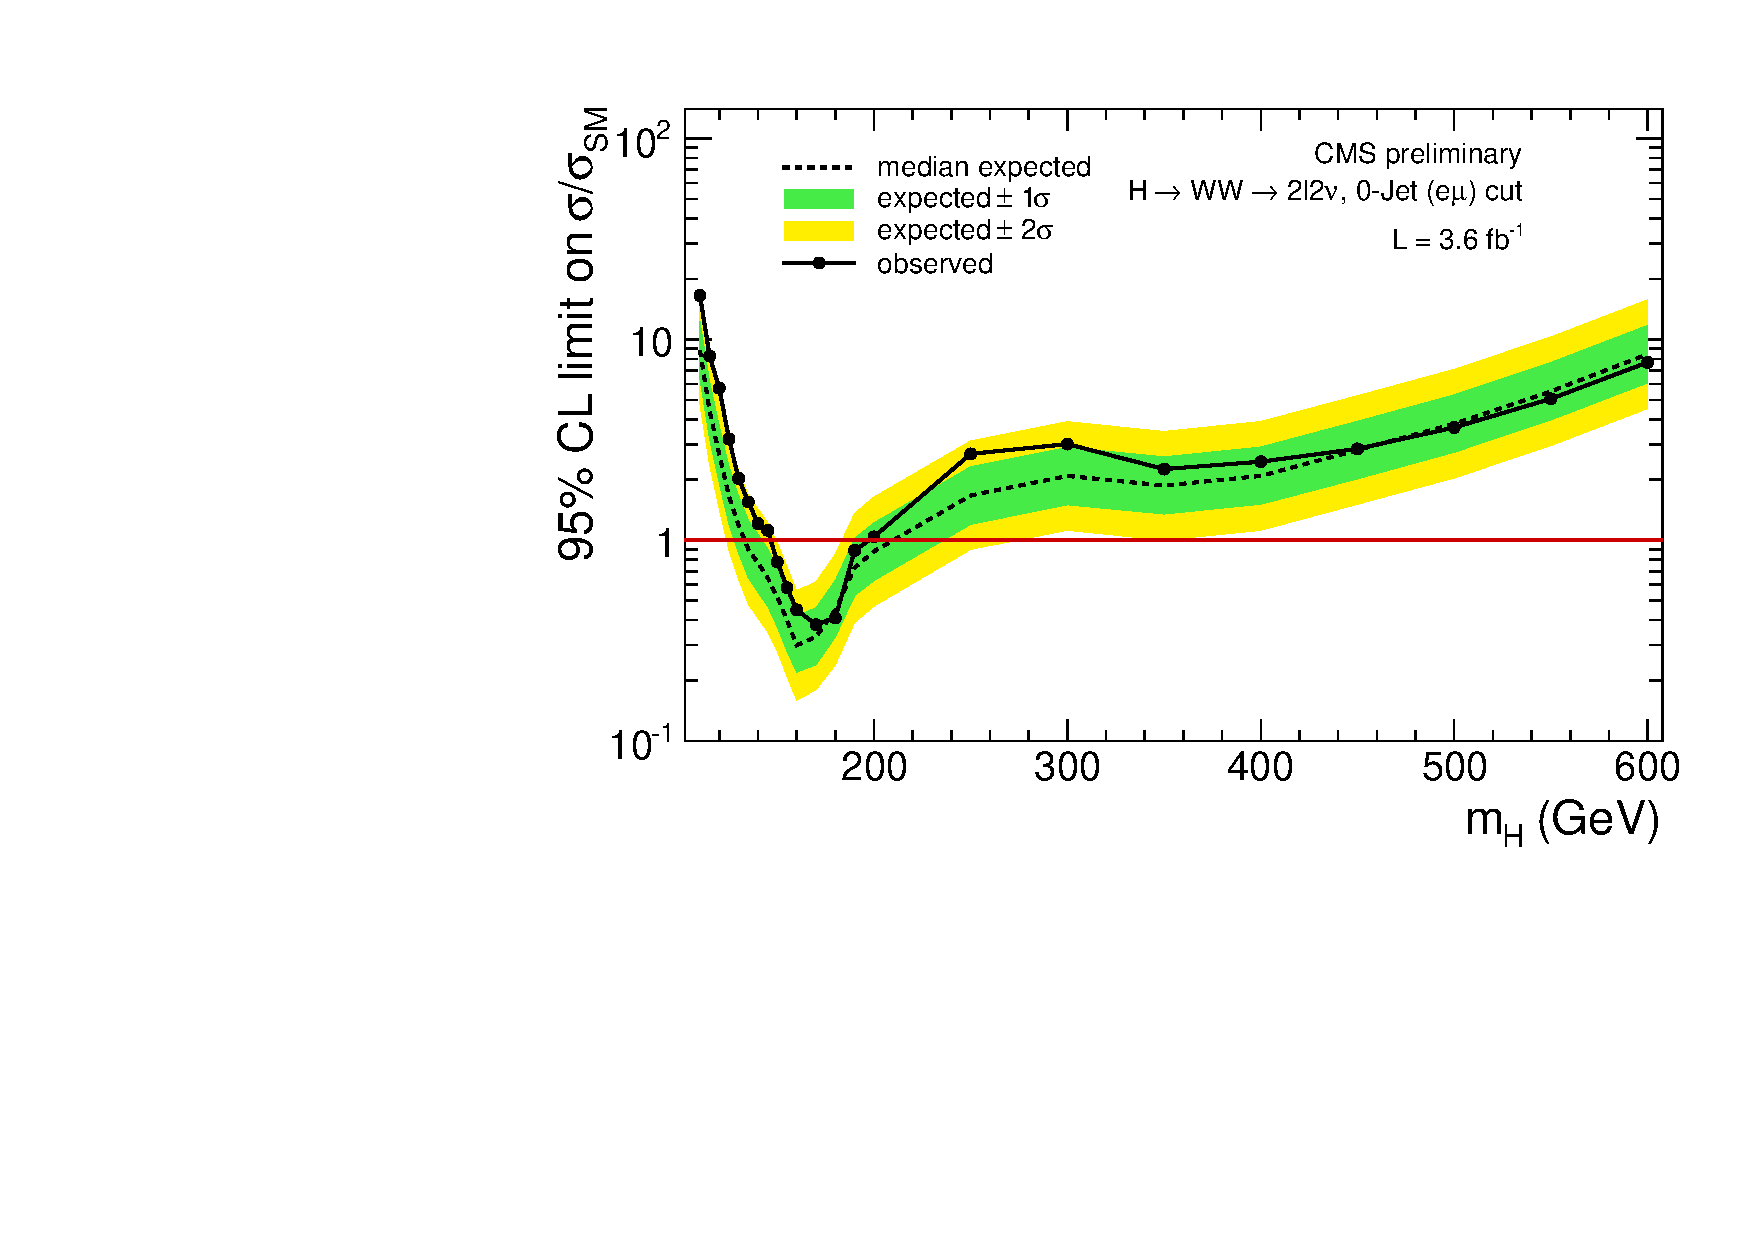
\includegraphics[width=.45\textwidth]{figures/limits_0jof_cut-CLs-asymptotic_log.pdf}}
\centering
\subfigure[cut-based 0-Jet OF (zoom)]{
\centering
\label{subfig:0jof_zoom_cut}
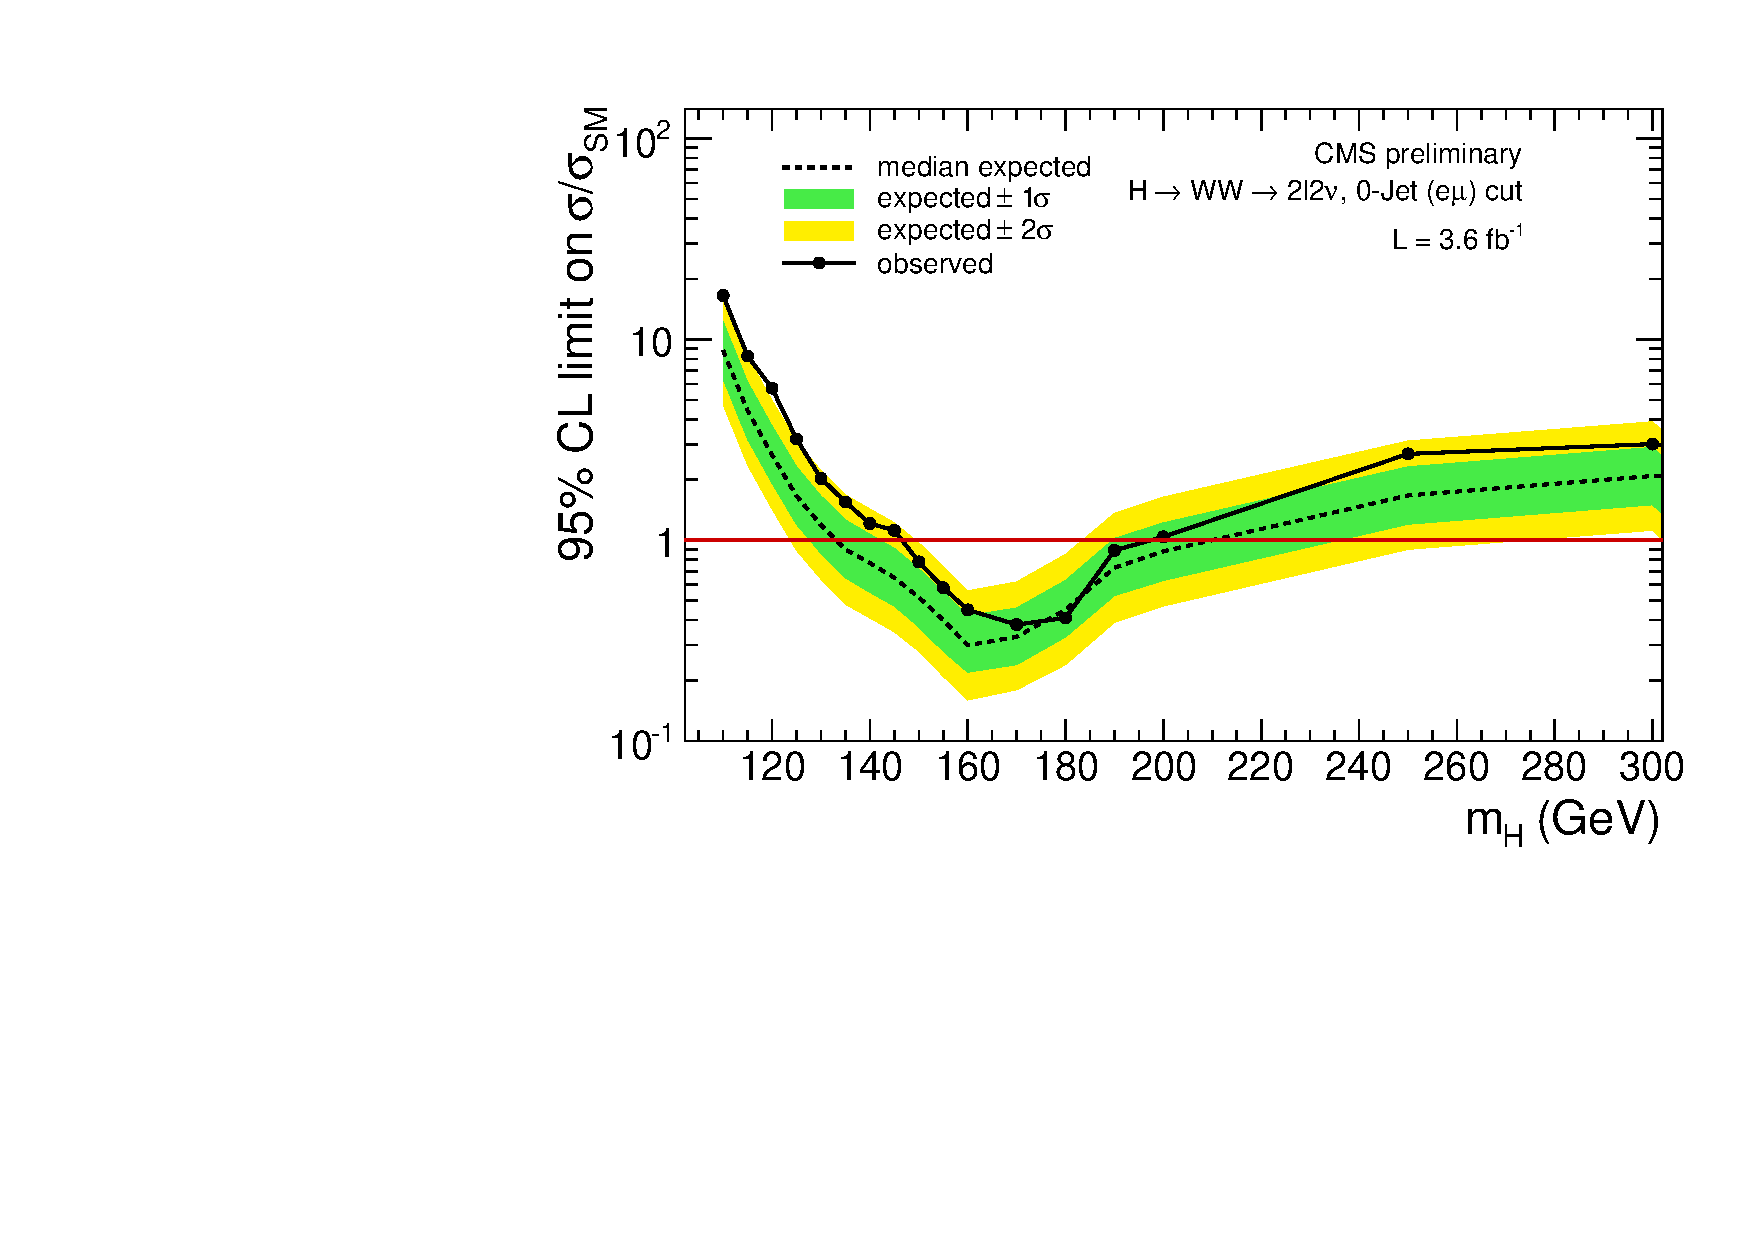
\includegraphics[width=.45\textwidth]{figures/limits_0jof_cut-CLs-asymptotic_zoom_log.pdf}} \\
\subfigure[cut-based 0-Jet SF]{
\centering
\label{subfig:0jsf_cut}
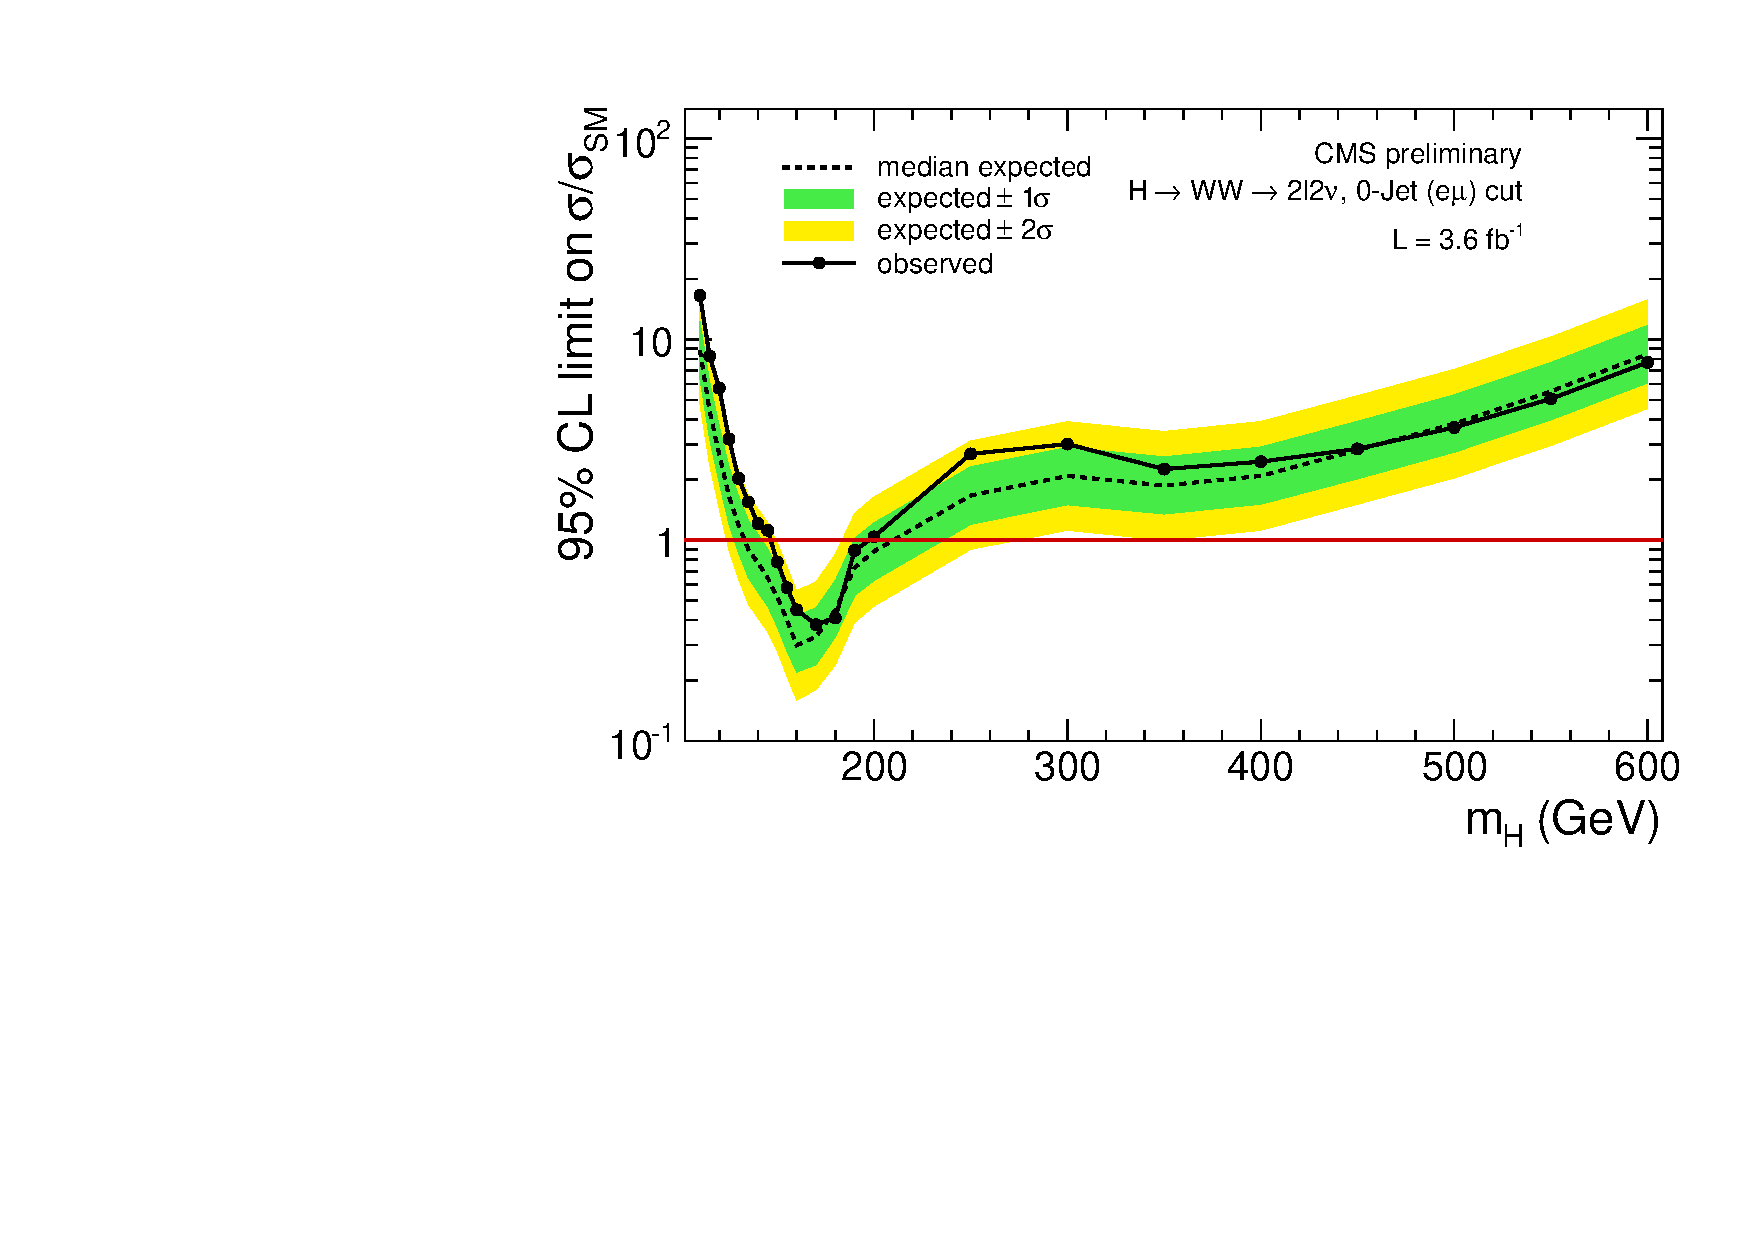
\includegraphics[width=.45\textwidth]{figures/limits_0jof_cut-CLs-asymptotic_log.pdf}}
\centering
\subfigure[cut-based 0-Jet SF (zoom)]{
\centering
\label{subfig:0jsf_zoom_cut}
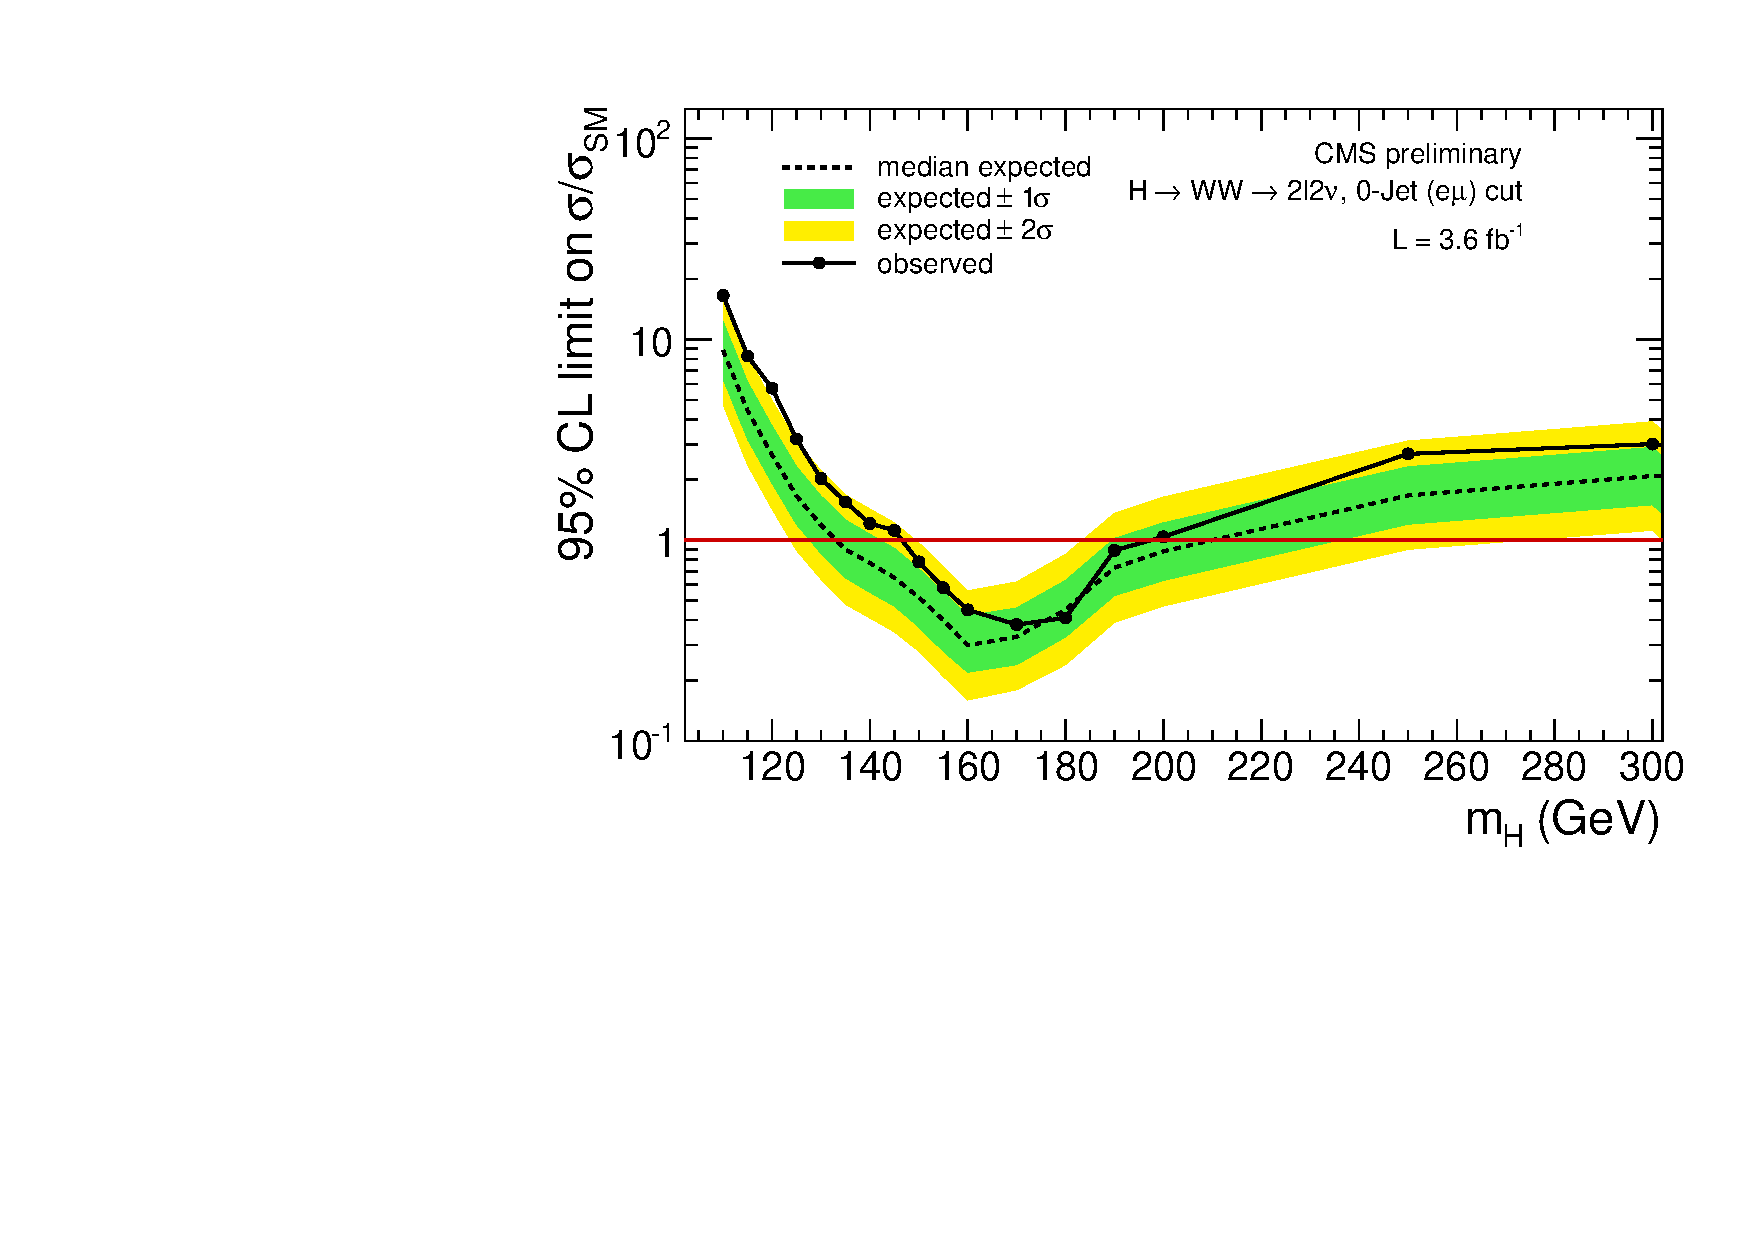
\includegraphics[width=.45\textwidth]{figures/limits_0jof_cut-CLs-asymptotic_zoom_log.pdf}} \\
\label{fig:uls_cut_0j}
\caption{The expected and observed limits for the Cut-based analysis for 3.5/fb in the {\bf 0-Jet bin} 
using the {\bf CLs-asymptotic} approach. }
\end{figure}
%%%%%%%%%%%%%%%%%%%%%%%%%%%%%%


%%%%%%%%%%%%%%%%%%%%%%%%%%%%%%
\begin{figure}[!hbtp]
\centering
\subfigure[cut-based 1-Jet OF]{
\centering
\label{subfig:1jof_cut}
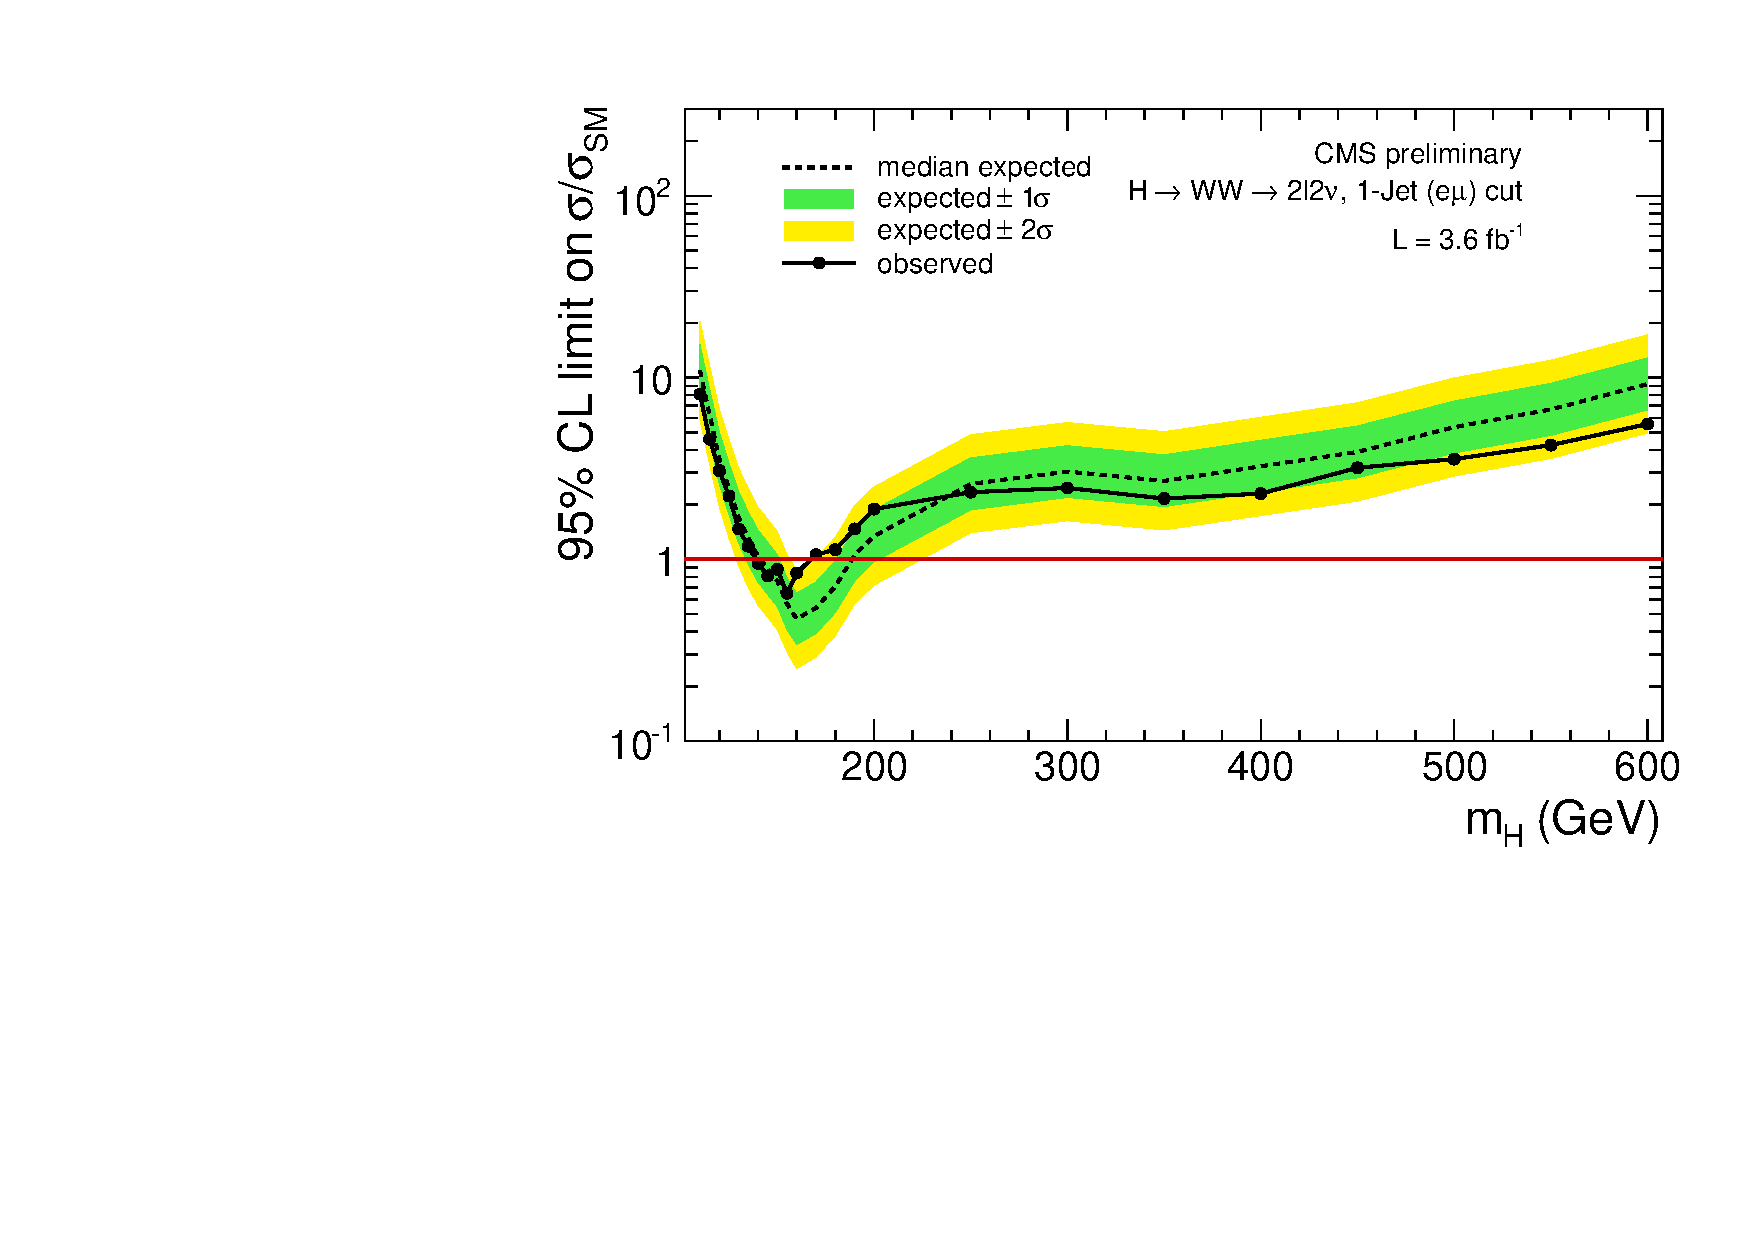
\includegraphics[width=.45\textwidth]{figures/limits_1jof_cut-CLs-asymptotic_log.pdf}}
\centering
\subfigure[cut-based 1-Jet OF (zoom)]{
\centering
\label{subfig:1jof_zoom_cut}
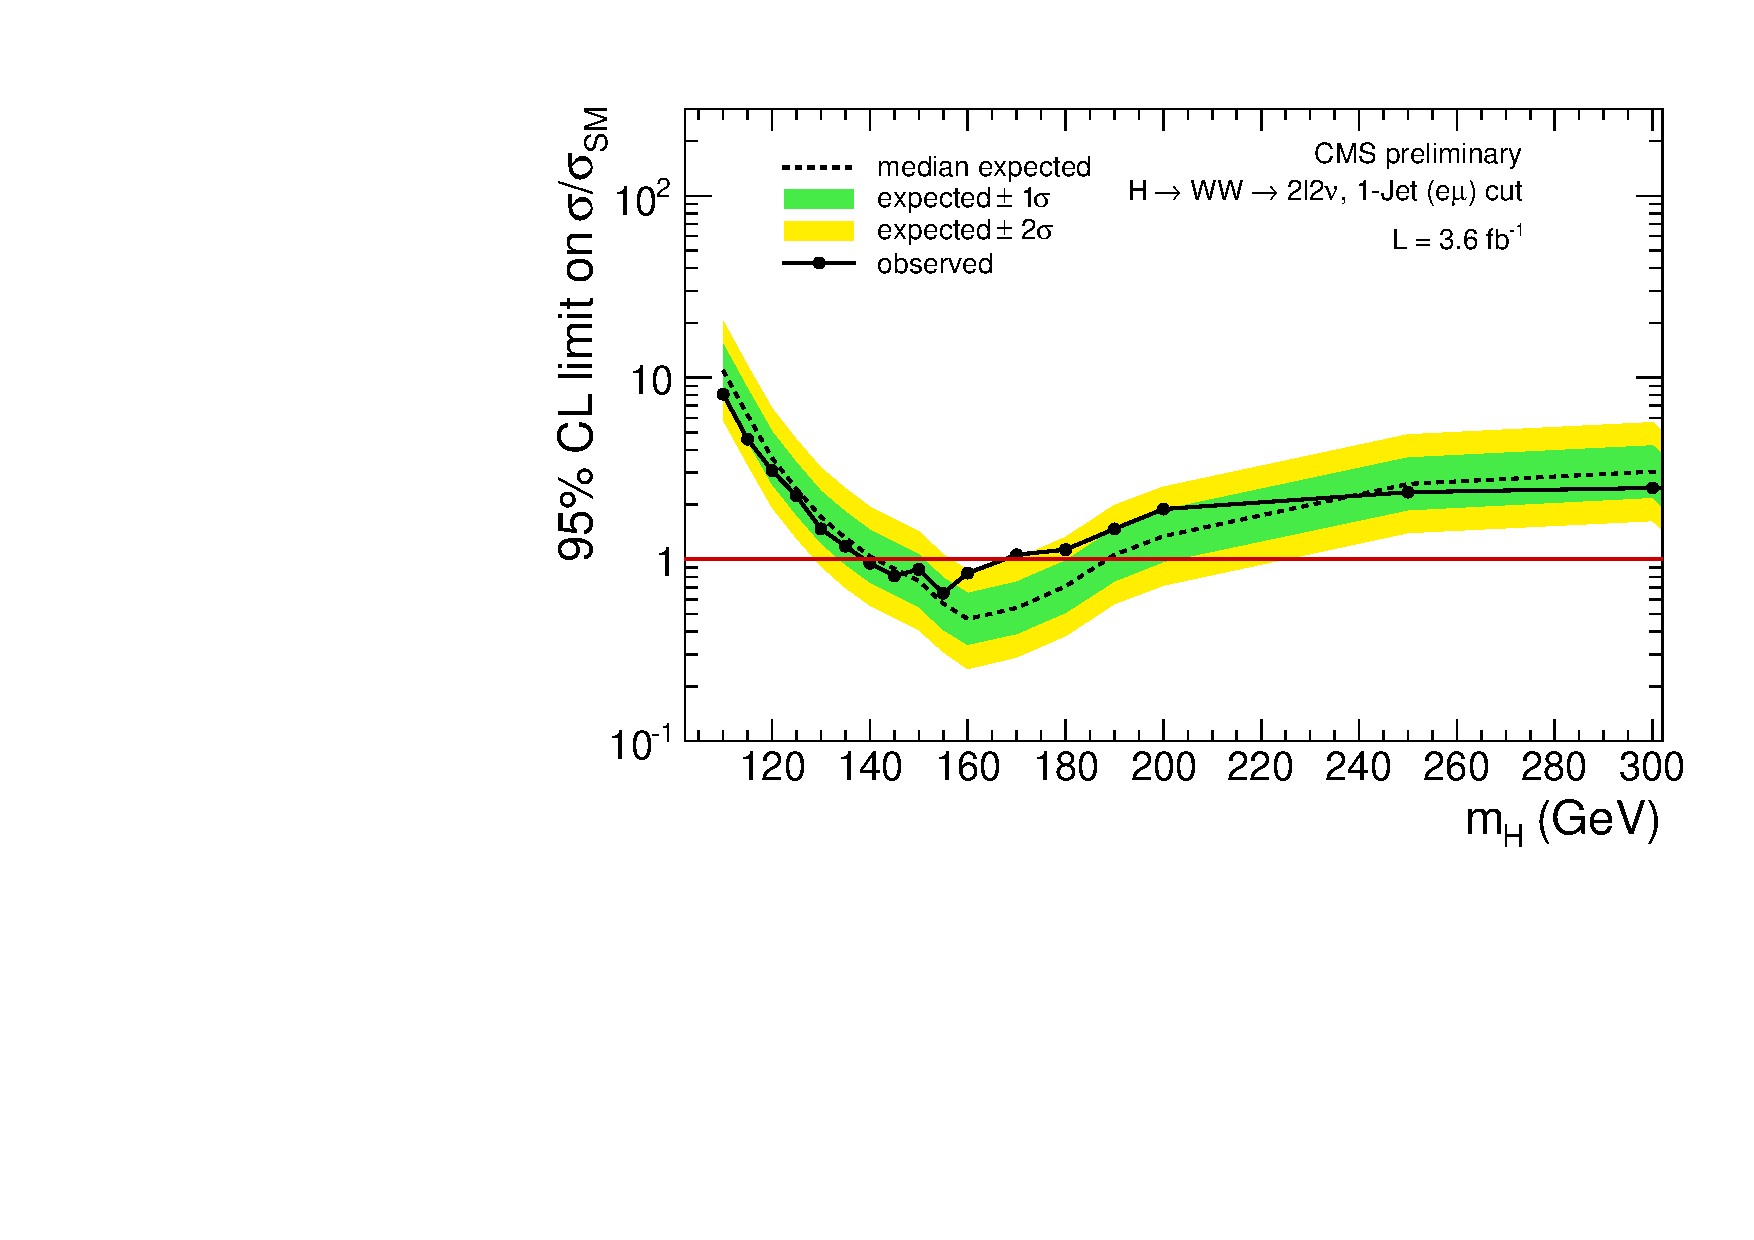
\includegraphics[width=.45\textwidth]{figures/limits_1jof_cut-CLs-asymptotic_zoom_log.pdf}} \\
\subfigure[cut-based 1-Jet SF]{
\centering
\label{subfig:1jsf_cut}
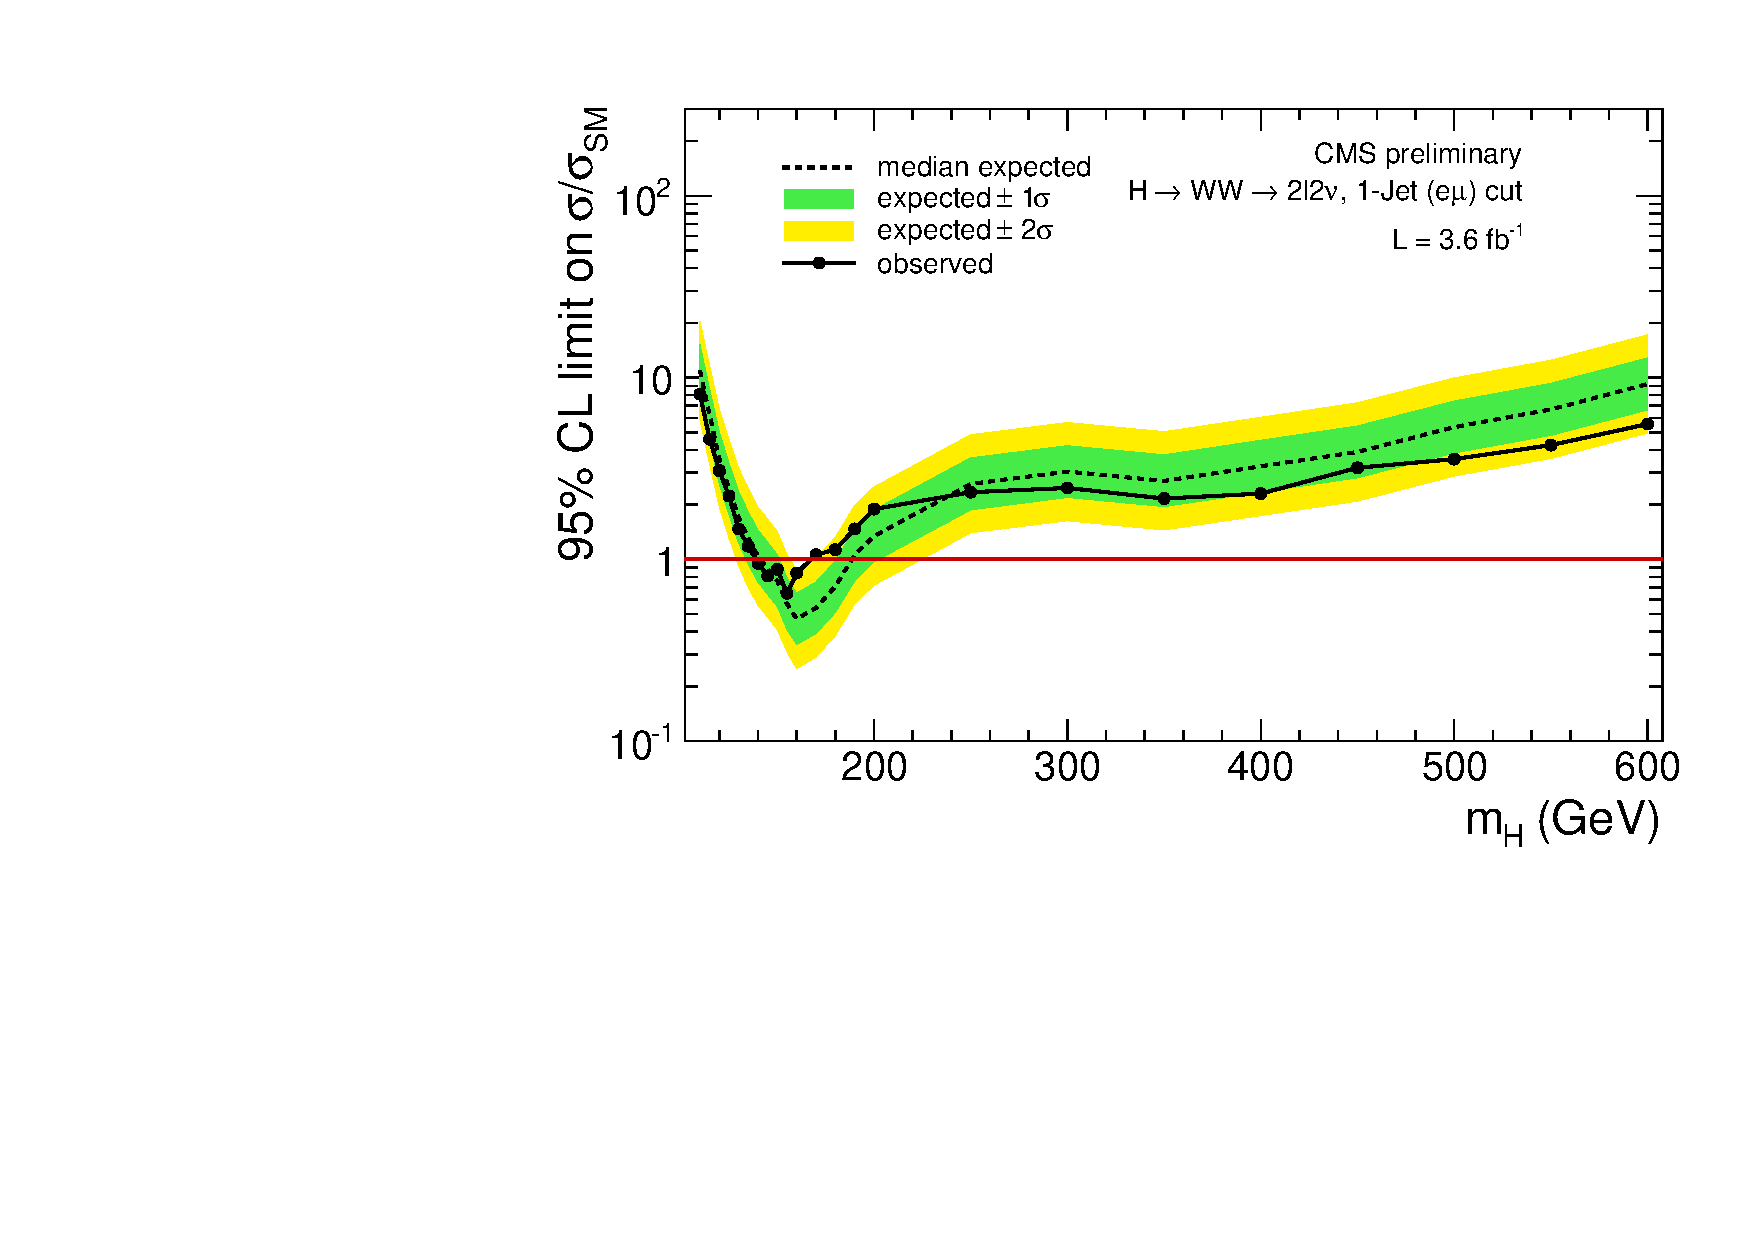
\includegraphics[width=.45\textwidth]{figures/limits_1jof_cut-CLs-asymptotic_log.pdf}}
\centering
\subfigure[cut-based 1-Jet SF (zoom)]{
\centering
\label{subfig:1jsf_zoom_cut}
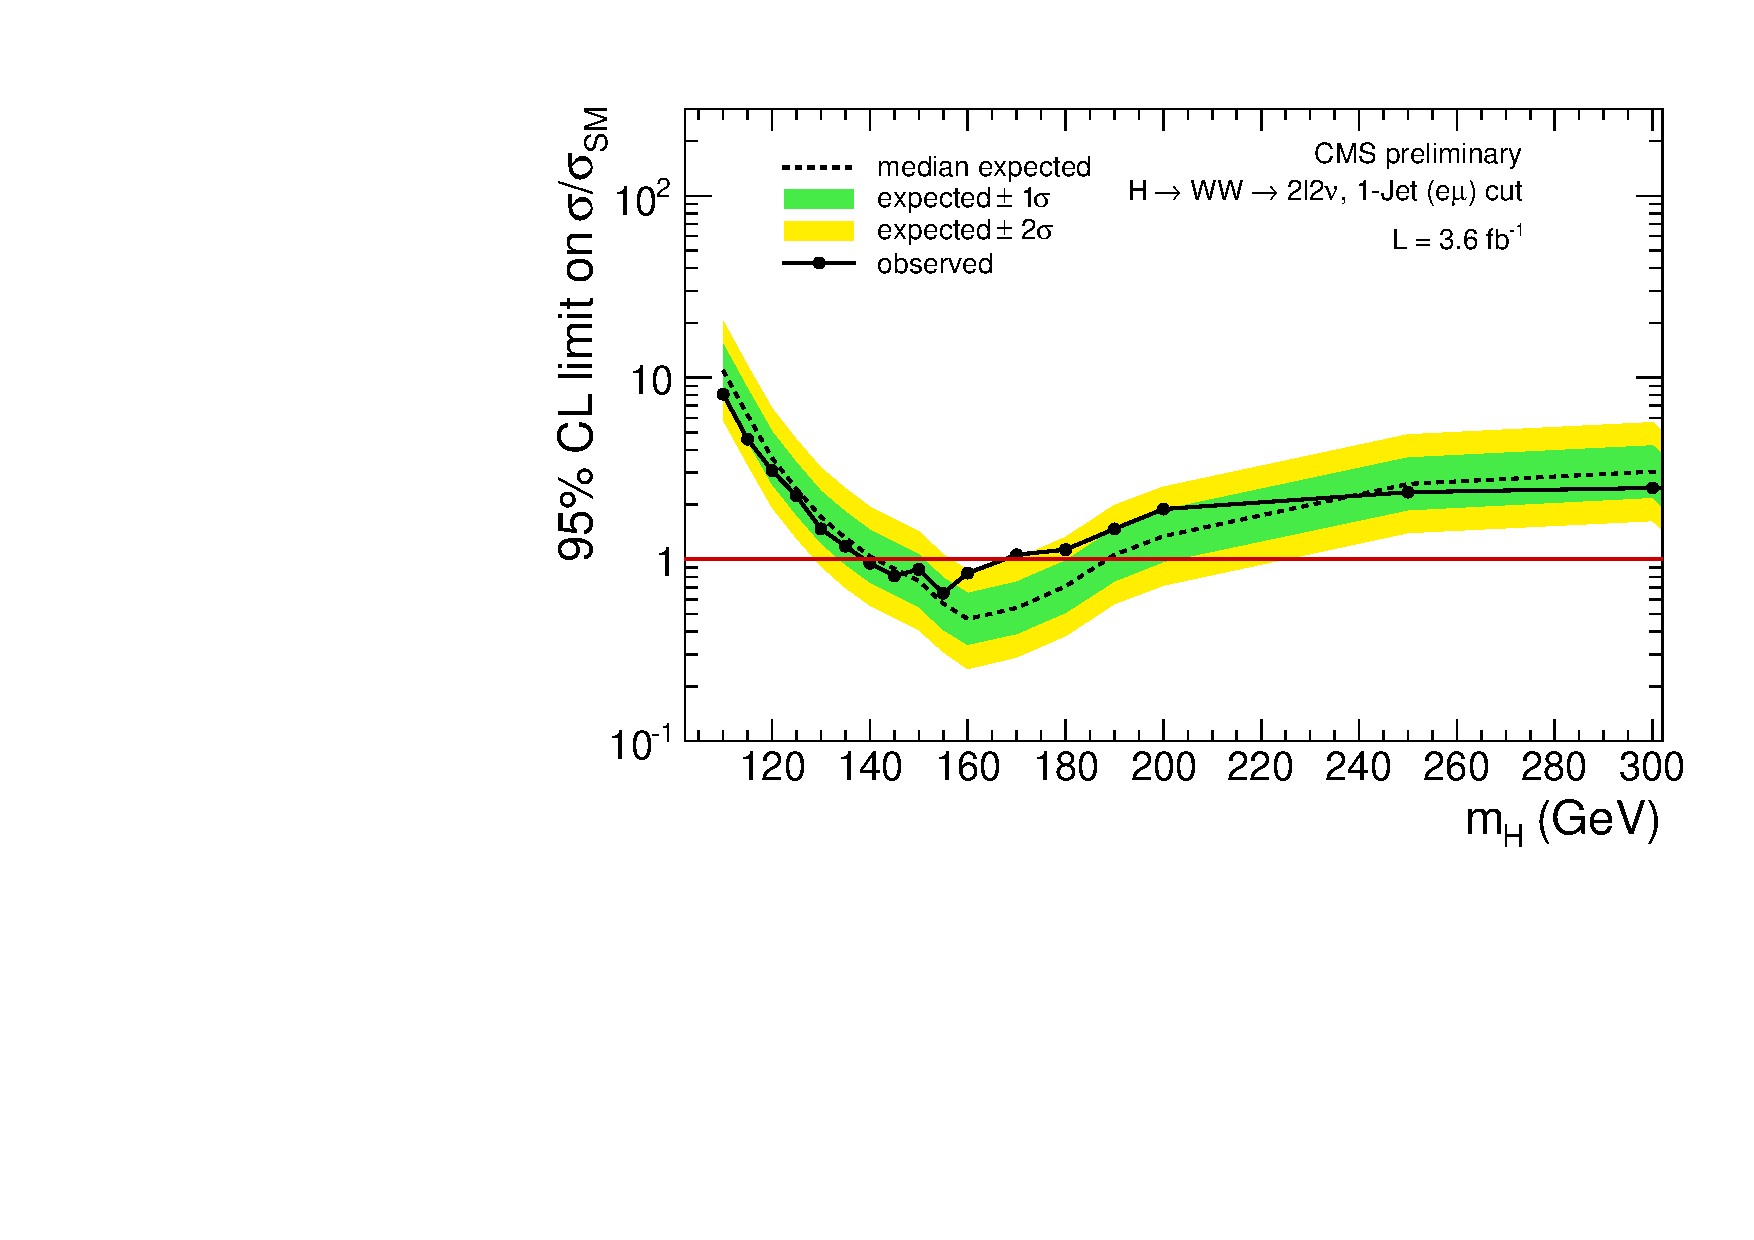
\includegraphics[width=.45\textwidth]{figures/limits_1jof_cut-CLs-asymptotic_zoom_log.pdf}} \\
\label{fig:uls_cut_1j}
\caption{The expected and observed limits for the Cut-based analysis for 3.5/fb in the {\bf 1-Jet bin} 
using the {\bf CLs-asymptotic} approach. }
\end{figure}
%%%%%%%%%%%%%%%%%%%%%%%%%%%%%%

%%%%%%%%%%%%%%%%%%%%%%%%%%%%%%
\begin{figure}[!hbtp]
\centering
\subfigure[cut-based 2-Jet]{
\centering
\label{subfig:2j_cut}
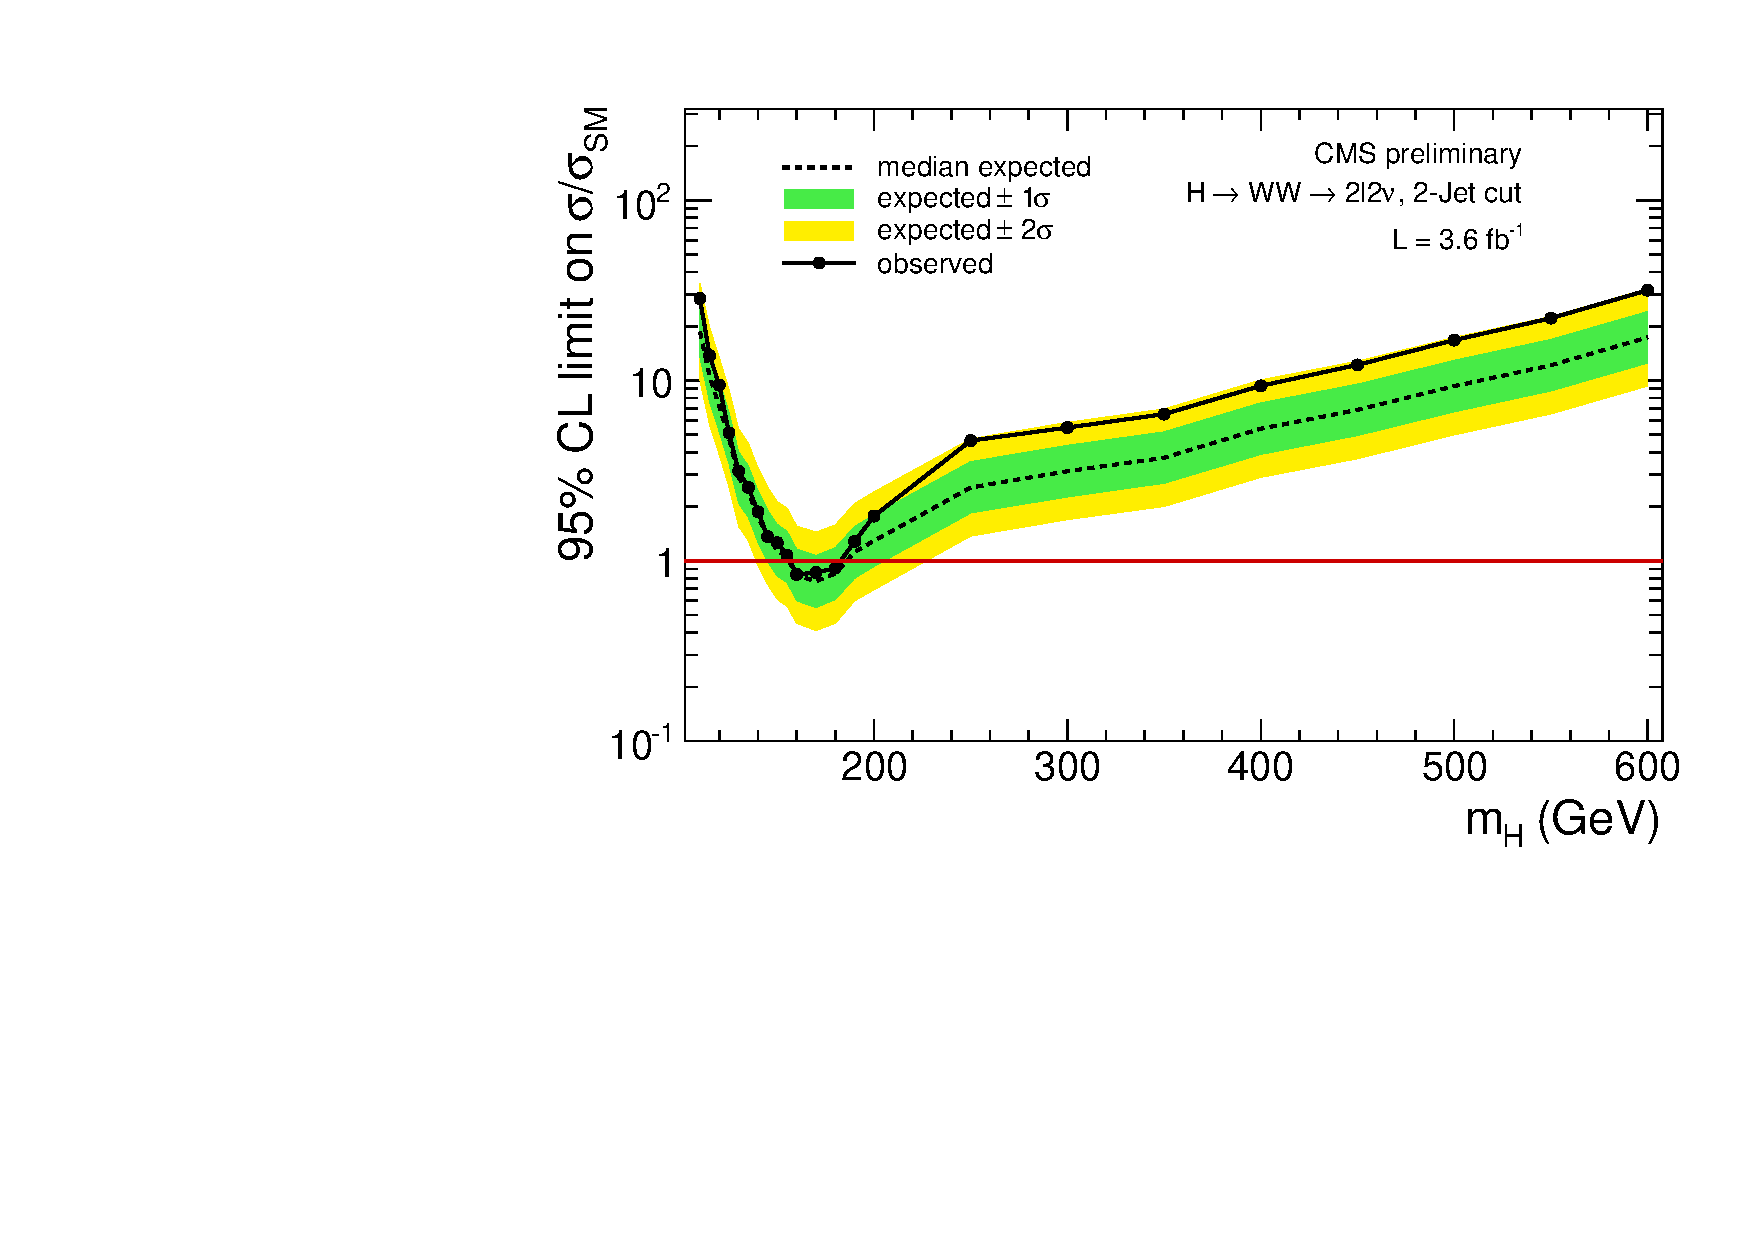
\includegraphics[width=.45\textwidth]{figures/limits_2j_cut-CLs-asymptotic_log.pdf}}
\centering
\subfigure[cut-based 2-Jet (zoom)]{
\centering
\label{subfig:2j_zoom_cut}
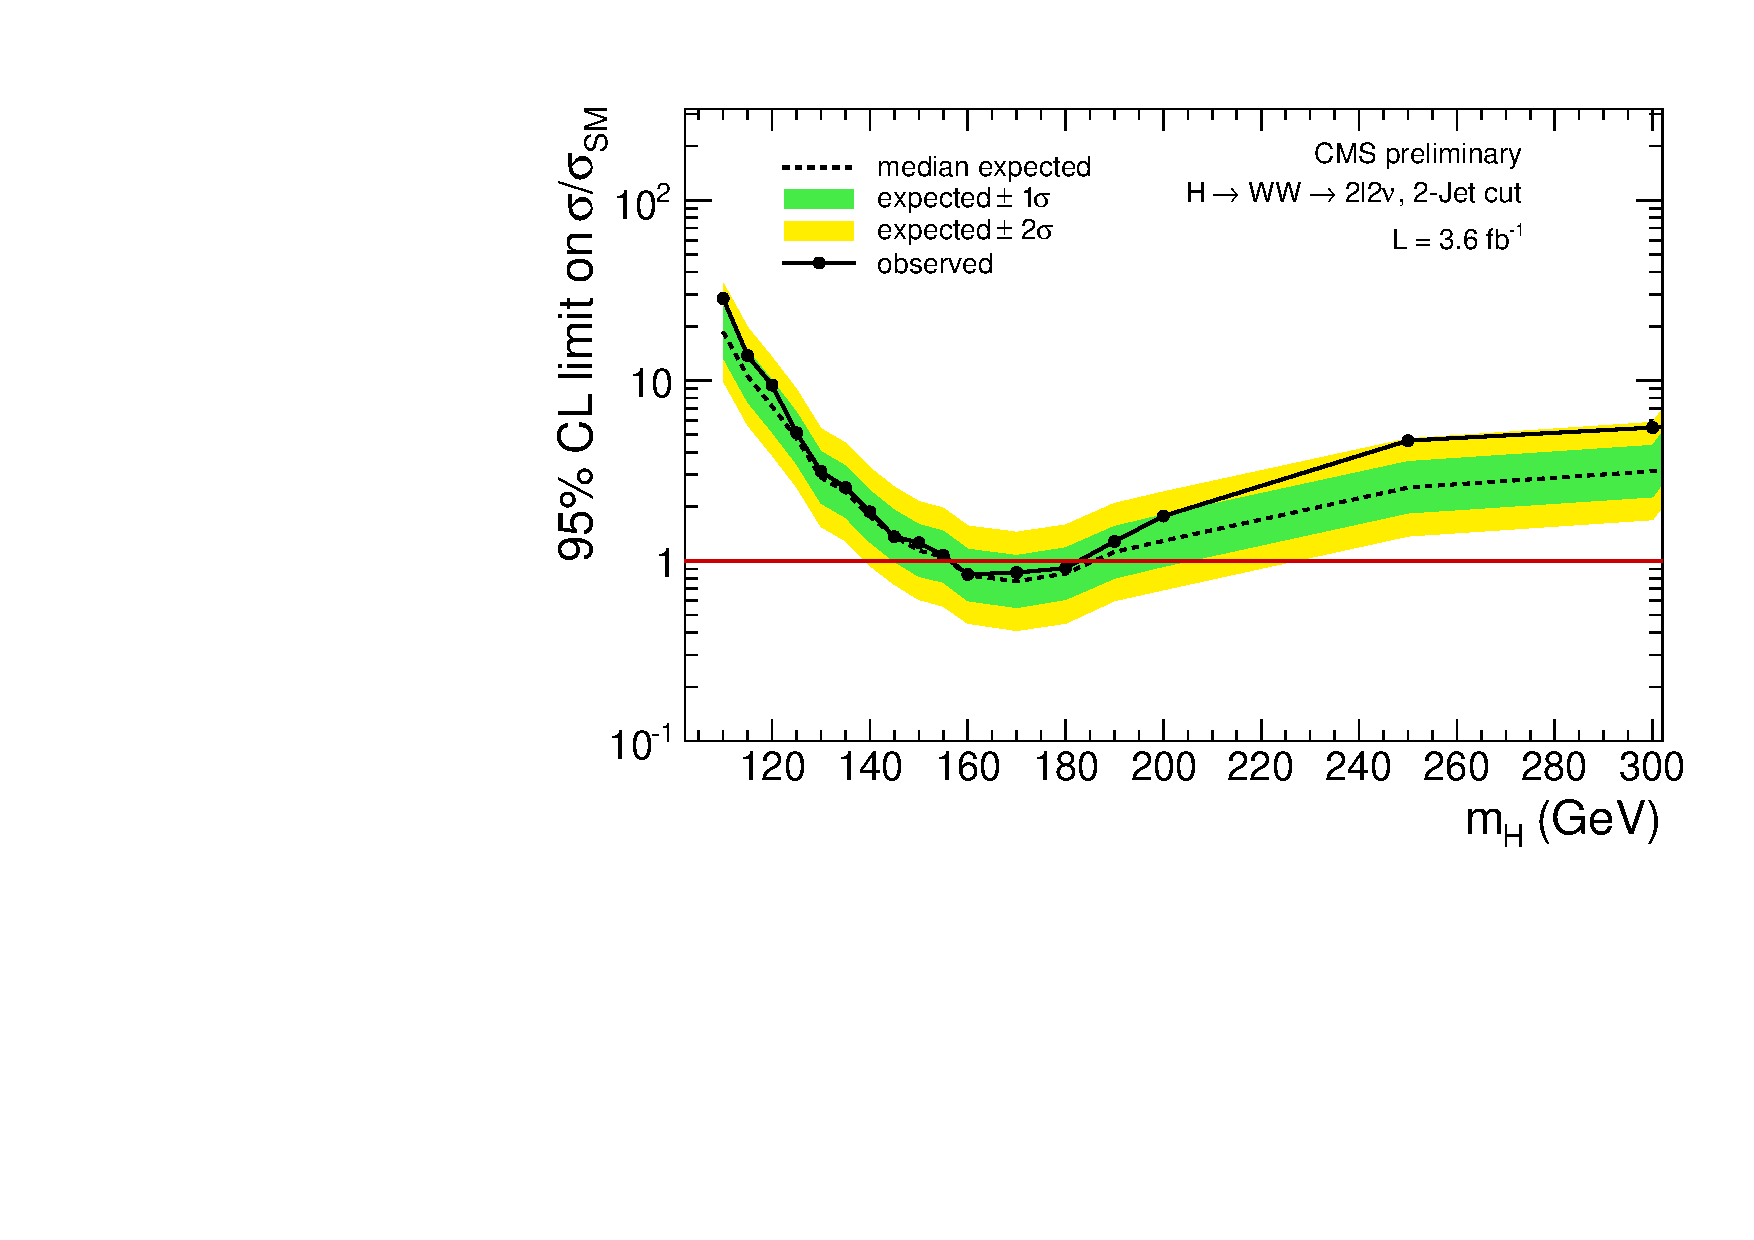
\includegraphics[width=.45\textwidth]{figures/limits_2j_cut-CLs-asymptotic_zoom_log.pdf}} \\
\label{fig:uls_cut_2j}
\caption{The expected and observed limits for the Cut-based analysis for 3.5/fb in the {\bf 2-Jet bin} 
using the {\bf CLs-asymptotic} approach. }
\end{figure}
%%%%%%%%%%%%%%%%%%%%%%%%%%%%%%


%%%%%%%%%%%%%%%%%%%%%%%%%%%%%%
\begin{table}[hbp!]
\begin{center}
\begin{tabular}{c c c c c}
\hline
\vspace{-3mm} && \\
 Higgs Mass & Observed  & Median expected & Expected range for 68\% & Expected range for 95\%   \\
\vspace{-3mm} && \\
\hline
110 & 16.6 & 8.8 & [6.3, 12.2] & [4.7, 16.4] \\
115 & 8.3 & 4.4 & [3.2, 6.1] & [2.4, 8.2] \\
120 & 5.7 & 2.7 & [1.9, 3.7] & [1.4, 5.0] \\
125 & 3.2 & 1.7 & [1.2, 2.3] & [0.9, 3.1] \\
130 & 2.0 & 1.2 & [0.9, 1.7] & [0.6, 2.2] \\
135 & 1.6 & 0.9 & [0.6, 1.3] & [0.5, 1.7] \\
140 & 1.2 & 0.8 & [0.6, 1.1] & [0.4, 1.4] \\
145 & 1.1 & 0.7 & [0.5, 0.9] & [0.4, 1.2] \\
150 & 0.8 & 0.5 & [0.4, 0.7] & [0.3, 1.0] \\
155 & 0.6 & 0.4 & [0.3, 0.5] & [0.2, 0.7] \\
160 & 0.5 & 0.3 & [0.2, 0.4] & [0.2, 0.6] \\
170 & 0.4 & 0.3 & [0.2, 0.5] & [0.2, 0.6] \\
180 & 0.4 & 0.5 & [0.3, 0.6] & [0.2, 0.8] \\
190 & 0.9 & 0.7 & [0.5, 1.0] & [0.4, 1.4] \\
200 & 1.1 & 0.9 & [0.6, 1.2] & [0.5, 1.6] \\
250 & 2.7 & 1.7 & [1.2, 2.3] & [0.9, 3.1] \\
300 & 3.0 & 2.1 & [1.5, 2.9] & [1.1, 3.9] \\
350 & 2.3 & 1.9 & [1.3, 2.6] & [1.0, 3.5] \\
400 & 2.5 & 2.1 & [1.5, 2.9] & [1.1, 3.9] \\
450 & 2.9 & 2.8 & [2.0, 3.9] & [1.5, 5.2] \\
500 & 3.7 & 3.8 & [2.7, 5.3] & [2.0, 7.1] \\
550 & 5.0 & 5.5 & [4.0, 7.6] & [2.9, 10.2] \\
600 & 7.7 & 8.4 & [6.1, 11.7] & [4.5, 15.7] \\
\hline
\end{tabular}
\caption{Expected and observed upper limits for SM Higgs using the
  {\bf cut-based} analysis in the {\bf $e\mu$ OF 0-Jet bin} with \intlumiEightTeV\ of data.}
\label{tab:cutbase_uls_0jof}
\end{center}
\end{table}
%%%%%%%%%%%%%%%%%%%%%%%%%%%%%%



%%%%%%%%%%%%%%%%%%%%%%%%%%%%%%
\begin{table}[hbp!]
\begin{center}
\begin{tabular}{c c c c c}
\hline
\vspace{-3mm} && \\
 Higgs Mass & Observed  & Median expected & Expected range for 68\% & Expected range for 95\%   \\
\vspace{-3mm} && \\
\hline
110 & 10.5 & 13.6 & [9.8, 19.0] & [7.3, 25.4] \\
115 & 5.7 & 7.2 & [5.2, 10.0] & [3.9, 13.4] \\
120 & 3.6 & 3.9 & [2.8, 5.4] & [2.1, 7.3] \\
125 & 3.4 & 2.6 & [1.9, 3.7] & [1.4, 4.9] \\
130 & 2.0 & 1.7 & [1.2, 2.4] & [0.9, 3.2] \\
135 & 1.4 & 1.4 & [1.0, 2.0] & [0.8, 2.6] \\
140 & 1.0 & 1.1 & [0.8, 1.5] & [0.6, 2.0] \\
145 & 1.4 & 0.8 & [0.6, 1.1] & [0.4, 1.4] \\
150 & 1.3 & 0.6 & [0.4, 0.8] & [0.3, 1.1] \\
155 & 0.8 & 0.4 & [0.3, 0.6] & [0.2, 0.7] \\
160 & 0.6 & 0.3 & [0.2, 0.4] & [0.2, 0.6] \\
170 & 0.6 & 0.3 & [0.2, 0.4] & [0.2, 0.6] \\
180 & 0.8 & 0.5 & [0.3, 0.7] & [0.3, 0.9] \\
190 & 1.3 & 0.7 & [0.5, 0.9] & [0.4, 1.2] \\
200 & 1.3 & 0.9 & [0.7, 1.3] & [0.5, 1.7] \\
250 & 1.2 & 1.8 & [1.3, 2.5] & [1.0, 3.4] \\
300 & 1.4 & 2.1 & [1.5, 3.0] & [1.1, 4.0] \\
350 & 1.0 & 1.7 & [1.2, 2.4] & [0.9, 3.2] \\
400 & 2.2 & 2.1 & [1.5, 2.9] & [1.1, 3.9] \\
450 & 1.9 & 2.7 & [2.0, 3.8] & [1.5, 5.1] \\
500 & 3.4 & 3.9 & [2.8, 5.4] & [2.1, 7.2] \\
550 & 6.0 & 5.6 & [4.0, 7.8] & [3.0, 10.4] \\
600 & 7.9 & 8.4 & [6.0, 11.6] & [4.5, 15.6] \\
\hline
\end{tabular}
\caption{Expected and observed upper limits for SM Higgs using the
  {\bf cut-based} analysis in the {\bf $ee/\mu\mu$ SF 0-Jet bin} with \intlumiEightTeV\ of data.}
\label{tab:cutbase_uls_0jsf}
\end{center}
\end{table}
%%%%%%%%%%%%%%%%%%%%%%%%%%%%%%
%%%%%%%%%%%%%%%%%%%%%%%%%%%%%%
\begin{table}[hbp!]
\begin{center}
\begin{tabular}{c c c c c}
\hline
\vspace{-3mm} && \\
 Higgs Mass & Observed  & Median expected & Expected range for 68\% & Expected range for 95\%   \\
\vspace{-3mm} && \\
\hline
110 & 8.1 & 10.9 & [7.9, 15.2] & [5.9, 20.4] \\
115 & 4.6 & 6.2 & [4.5, 8.7] & [3.3, 11.6] \\
120 & 3.1 & 3.6 & [2.6, 5.0] & [1.9, 6.7] \\
125 & 2.2 & 2.4 & [1.8, 3.4] & [1.3, 4.5] \\
130 & 1.5 & 1.7 & [1.2, 2.4] & [0.9, 3.2] \\
135 & 1.2 & 1.3 & [0.9, 1.8] & [0.7, 2.4] \\
140 & 1.0 & 1.0 & [0.7, 1.4] & [0.6, 1.9] \\
145 & 0.8 & 0.9 & [0.6, 1.2] & [0.5, 1.7] \\
150 & 0.9 & 0.8 & [0.5, 1.1] & [0.4, 1.4] \\
155 & 0.6 & 0.6 & [0.4, 0.8] & [0.3, 1.1] \\
160 & 0.8 & 0.5 & [0.3, 0.7] & [0.3, 0.9] \\
170 & 1.1 & 0.5 & [0.4, 0.8] & [0.3, 1.0] \\
180 & 1.1 & 0.7 & [0.5, 1.0] & [0.4, 1.3] \\
190 & 1.5 & 1.1 & [0.8, 1.5] & [0.6, 2.0] \\
200 & 1.9 & 1.3 & [1.0, 1.9] & [0.7, 2.5] \\
250 & 2.3 & 2.6 & [1.9, 3.6] & [1.4, 4.9] \\
300 & 2.5 & 3.0 & [2.2, 4.2] & [1.6, 5.7] \\
350 & 2.2 & 2.7 & [1.9, 3.8] & [1.5, 5.0] \\
400 & 2.3 & 3.2 & [2.3, 4.5] & [1.7, 6.1] \\
450 & 3.2 & 3.9 & [2.8, 5.4] & [2.1, 7.3] \\
500 & 3.6 & 5.3 & [3.8, 7.4] & [2.9, 10.0] \\
550 & 4.2 & 6.7 & [4.8, 9.3] & [3.6, 12.5] \\
600 & 5.6 & 9.2 & [6.6, 12.8] & [4.9, 17.2] \\

\vspace{-3mm} && \\
\hline
\hline
\end{tabular}
\caption{Expected and observed upper limits for SM Higgs using the
  {\bf cut-based} analysis in the {\bf $ee/\mu\mu$ OF 1-Jet bin} with \intlumiEightTeV\ of data.}
\label{tab:cutbase_uls_1jof}
\end{center}
\end{table}
%%%%%%%%%%%%%%%%%%%%%%%%%%%%%%


%%%%%%%%%%%%%%%%%%%%%%%%%%%%%%
\begin{table}[hbp!]
\begin{center}
\begin{tabular}{c c c c c}
\hline
\vspace{-3mm} && \\
 Higgs Mass & Observed  & Median expected & Expected range for 68\% & Expected range for 95\%   \\
\vspace{-3mm} && \\
\hline
110 & 15.5 & 22.9 & [16.5, 31.9] & [12.3, 42.8] \\
115 & 9.9 & 14.6 & [10.5, 20.4] & [7.9, 27.3] \\
120 & 6.3 & 7.3 & [5.2, 10.1] & [3.9, 13.5] \\
125 & 4.1 & 4.3 & [3.1, 6.0] & [2.3, 8.0] \\
130 & 3.2 & 2.9 & [2.1, 4.1] & [1.6, 5.5] \\
135 & 2.8 & 2.4 & [1.7, 3.4] & [1.3, 4.5] \\
140 & 2.4 & 1.9 & [1.4, 2.6] & [1.0, 3.5] \\
145 & 2.2 & 2.0 & [1.5, 2.8] & [1.1, 3.8] \\
150 & 1.9 & 1.5 & [1.1, 2.1] & [0.8, 2.9] \\
155 & 1.4 & 1.1 & [0.8, 1.6] & [0.6, 2.1] \\
160 & 0.8 & 0.7 & [0.5, 1.0] & [0.4, 1.3] \\
170 & 1.1 & 0.9 & [0.6, 1.2] & [0.5, 1.7] \\
180 & 1.5 & 1.2 & [0.8, 1.6] & [0.6, 2.2] \\
190 & 2.8 & 1.8 & [1.3, 2.6] & [1.0, 3.4] \\
200 & 4.1 & 2.3 & [1.7, 3.2] & [1.2, 4.3] \\
250 & 6.0 & 4.2 & [3.0, 5.8] & [2.2, 7.7] \\
300 & 3.4 & 4.2 & [3.0, 5.8] & [2.2, 7.8] \\
350 & 2.5 & 3.2 & [2.3, 4.5] & [1.7, 6.0] \\
400 & 2.9 & 3.8 & [2.8, 5.3] & [2.1, 7.1] \\
450 & 3.6 & 5.2 & [3.7, 7.2] & [2.8, 9.6] \\
500 & 4.7 & 7.0 & [5.0, 9.7] & [3.8, 13.0] \\
550 & 6.6 & 8.7 & [6.3, 12.1] & [4.7, 16.2] \\
600 & 9.7 & 13.2 & [9.5, 18.3] & [7.1, 24.6] \\
\hline
\end{tabular}
\caption{Expected and observed upper limits for SM Higgs using the
  {\bf cut-based} analysis in the {\bf $ee/\mu\mu$ SF 1-Jet bin} with \intlumiEightTeV\ of data.}
\label{tab:cutbase_uls_1jsf}
\end{center}
\end{table}
%%%%%%%%%%%%%%%%%%%%%%%%%%%%%%


%%%%%%%%%%%%%%%%%%%%%%%%%%%%%%
\begin{table}[hbp!]
\begin{center}
\begin{tabular}{c c c c c}
\hline
\vspace{-3mm} && \\
 Higgs Mass & observed  & Median expected & Expected range for 68\% & Expected range for 95\%   \\
\vspace{-3mm} && \\
\hline
110 & 28.5 & 18.6 & [13.4, 25.9] & [10.0, 34.7] \\
115 & 13.7 & 10.6 & [7.6, 14.7] & [5.7, 19.7] \\
120 & 9.4 & 7.2 & [5.2, 10.0] & [3.9, 13.4] \\
125 & 5.1 & 4.8 & [3.4, 6.7] & [2.6, 8.9] \\
130 & 3.1 & 2.9 & [2.1, 4.0] & [1.6, 5.4] \\
135 & 2.6 & 2.4 & [1.7, 3.4] & [1.3, 4.5] \\
140 & 1.9 & 1.8 & [1.3, 2.4] & [0.9, 3.3] \\
145 & 1.4 & 1.4 & [1.0, 1.9] & [0.7, 2.6] \\
150 & 1.3 & 1.1 & [0.8, 1.6] & [0.6, 2.1] \\
155 & 1.1 & 1.0 & [0.8, 1.5] & [0.6, 2.0] \\
160 & 0.8 & 0.8 & [0.6, 1.2] & [0.4, 1.6] \\
170 & 0.9 & 0.8 & [0.6, 1.1] & [0.4, 1.4] \\
180 & 0.9 & 0.8 & [0.6, 1.2] & [0.5, 1.6] \\
190 & 1.3 & 1.1 & [0.8, 1.6] & [0.6, 2.1] \\
200 & 1.8 & 1.3 & [0.9, 1.8] & [0.7, 2.4] \\
250 & 4.6 & 2.5 & [1.8, 3.5] & [1.4, 4.8] \\
300 & 5.5 & 3.1 & [2.3, 4.4] & [1.7, 5.9] \\
350 & 6.5 & 3.7 & [2.7, 5.2] & [2.0, 7.0] \\
400 & 9.3 & 5.4 & [3.9, 7.5] & [2.9, 10.1] \\
450 & 12.2 & 6.9 & [4.9, 9.6] & [3.7, 12.8] \\
500 & 16.7 & 9.3 & [6.7, 12.9] & [5.0, 17.3] \\
550 & 22.2 & 12.1 & [8.8, 16.9] & [6.5, 22.7] \\
600 & 31.7 & 17.3 & [12.5, 24.1] & [9.3, 32.3] \\
\hline
\end{tabular}
\caption{Expected and observed upper limits for SM Higgs using the
  {\bf cut-based} analysis in the {\bf 2-Jet bin} with \intlumiEightTeV\ of data for the 
 masses that have VBF MC available. }
\label{tab:cutbase_uls_2j}
\end{center}
\end{table}
\clearpage


\subsection{Shape-based Analysis}
Figure~\ref{fig:uls_shape_0j}-\ref{fig:uls_shape_1j} show the expected and observed limits in the cut-based analysis 
for all contributing final states with the numbers tablulated in Table~\ref{tab:bdtbase_uls_0jof}-\ref{tab:bdtbase_uls_1jsf}. 


%%%%%%%%%%%%%%%%%%%%%%%%%%%%%%
\begin{figure}[!hbtp]
\centering
\subfigure[shape-based 0-Jet OF]{
\centering
\label{subfig:0jof_shape}
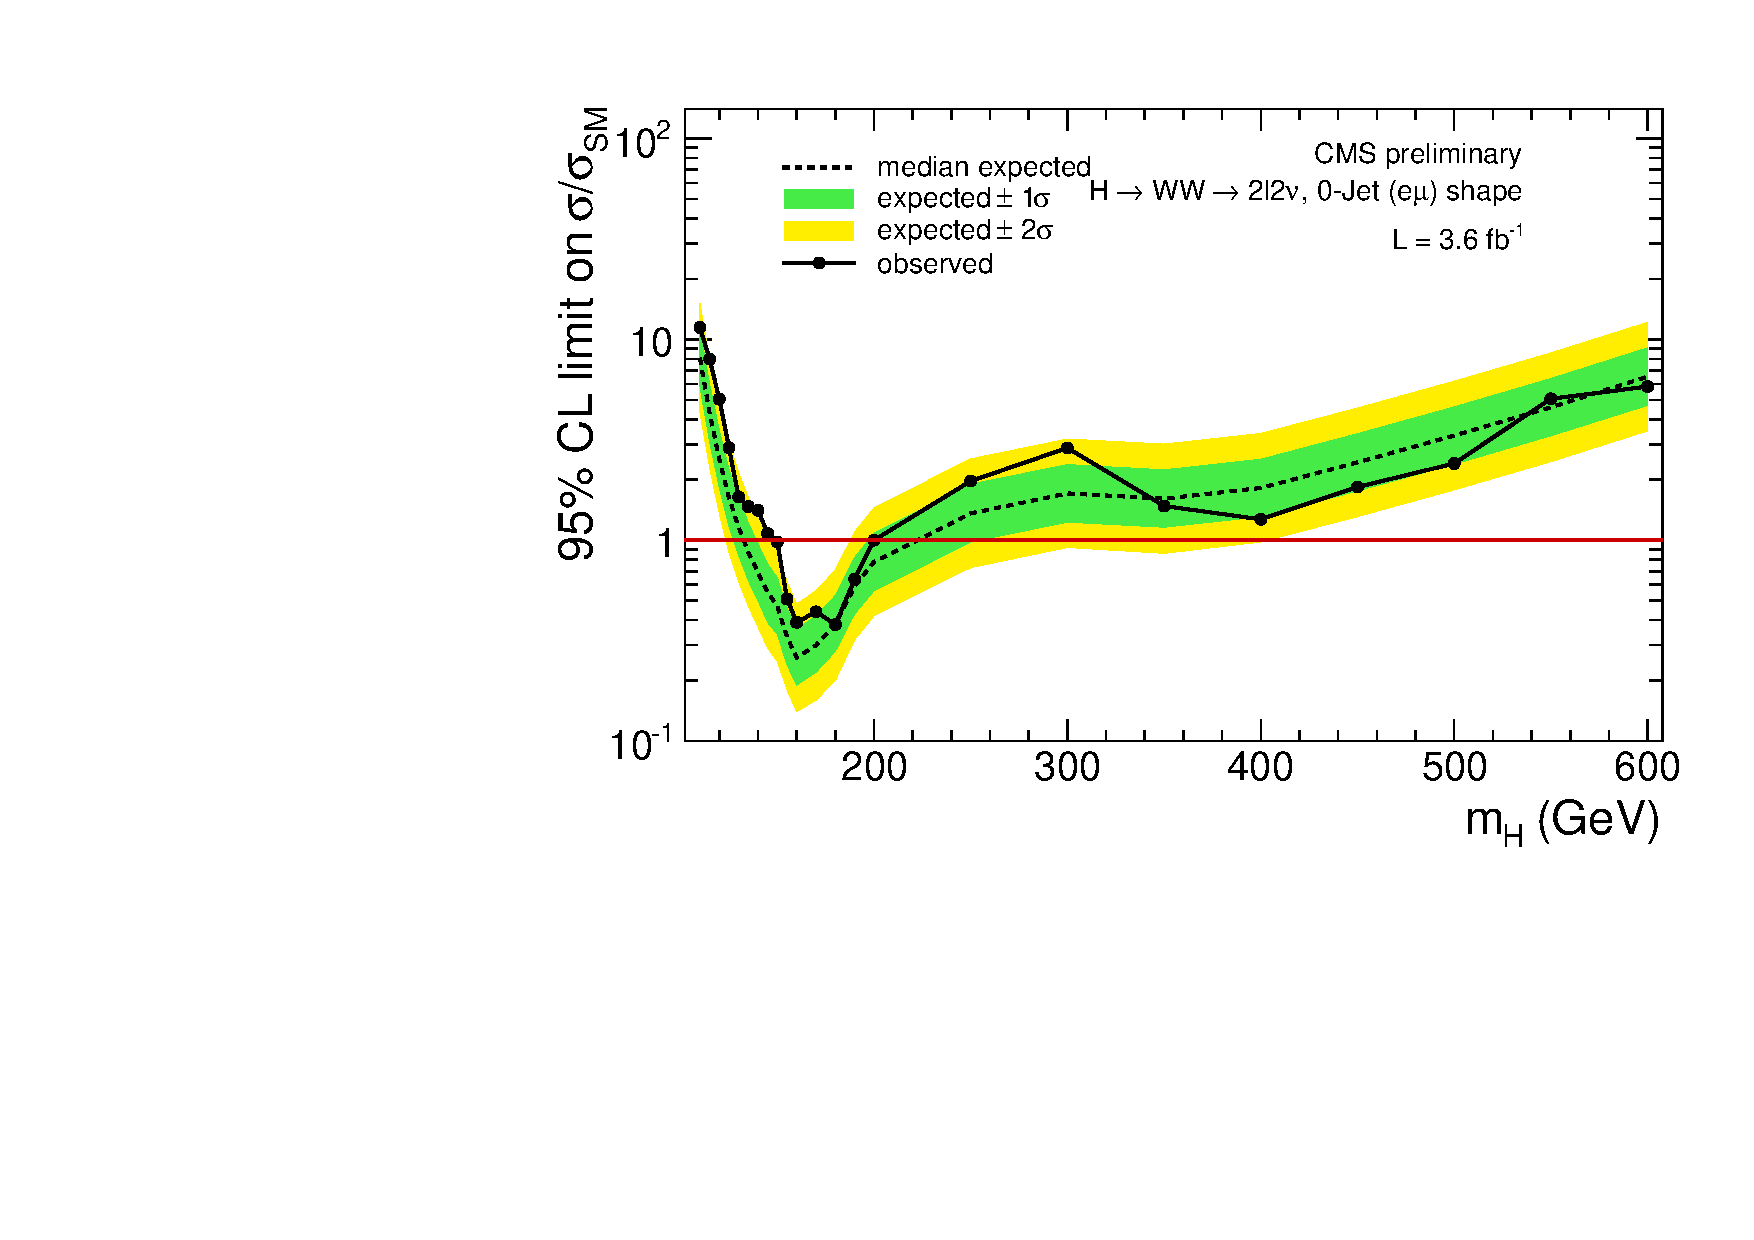
\includegraphics[width=.45\textwidth]{figures/limits_0jof_shape-CLs-asymptotic_log.pdf}}
\centering
\subfigure[shape-based 0-Jet OF (zoom)]{
\centering
\label{subfig:0jof_zoom_shape}
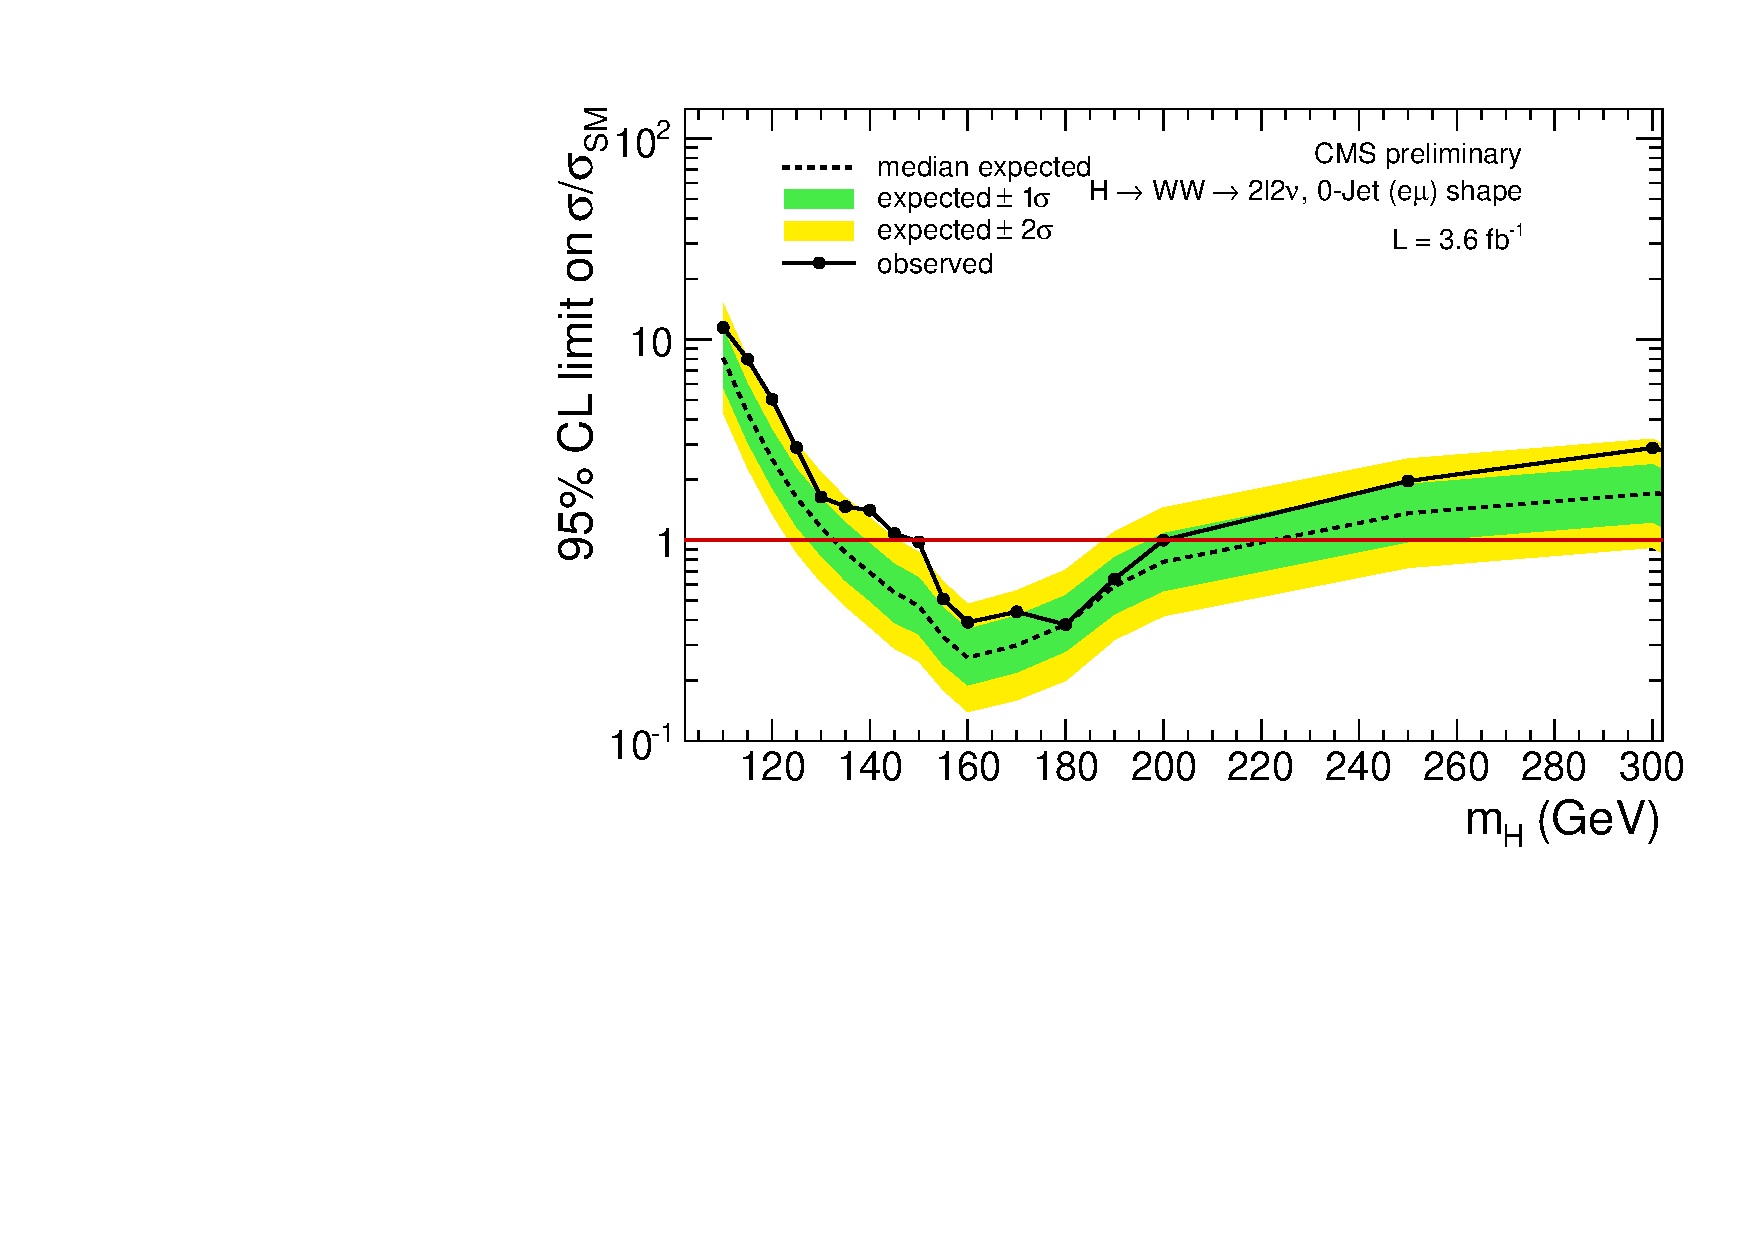
\includegraphics[width=.45\textwidth]{figures/limits_0jof_shape-CLs-asymptotic_zoom_log.pdf}} \\
\subfigure[shape-based 0-Jet SF]{
\centering
\label{subfig:0jsf_shape}
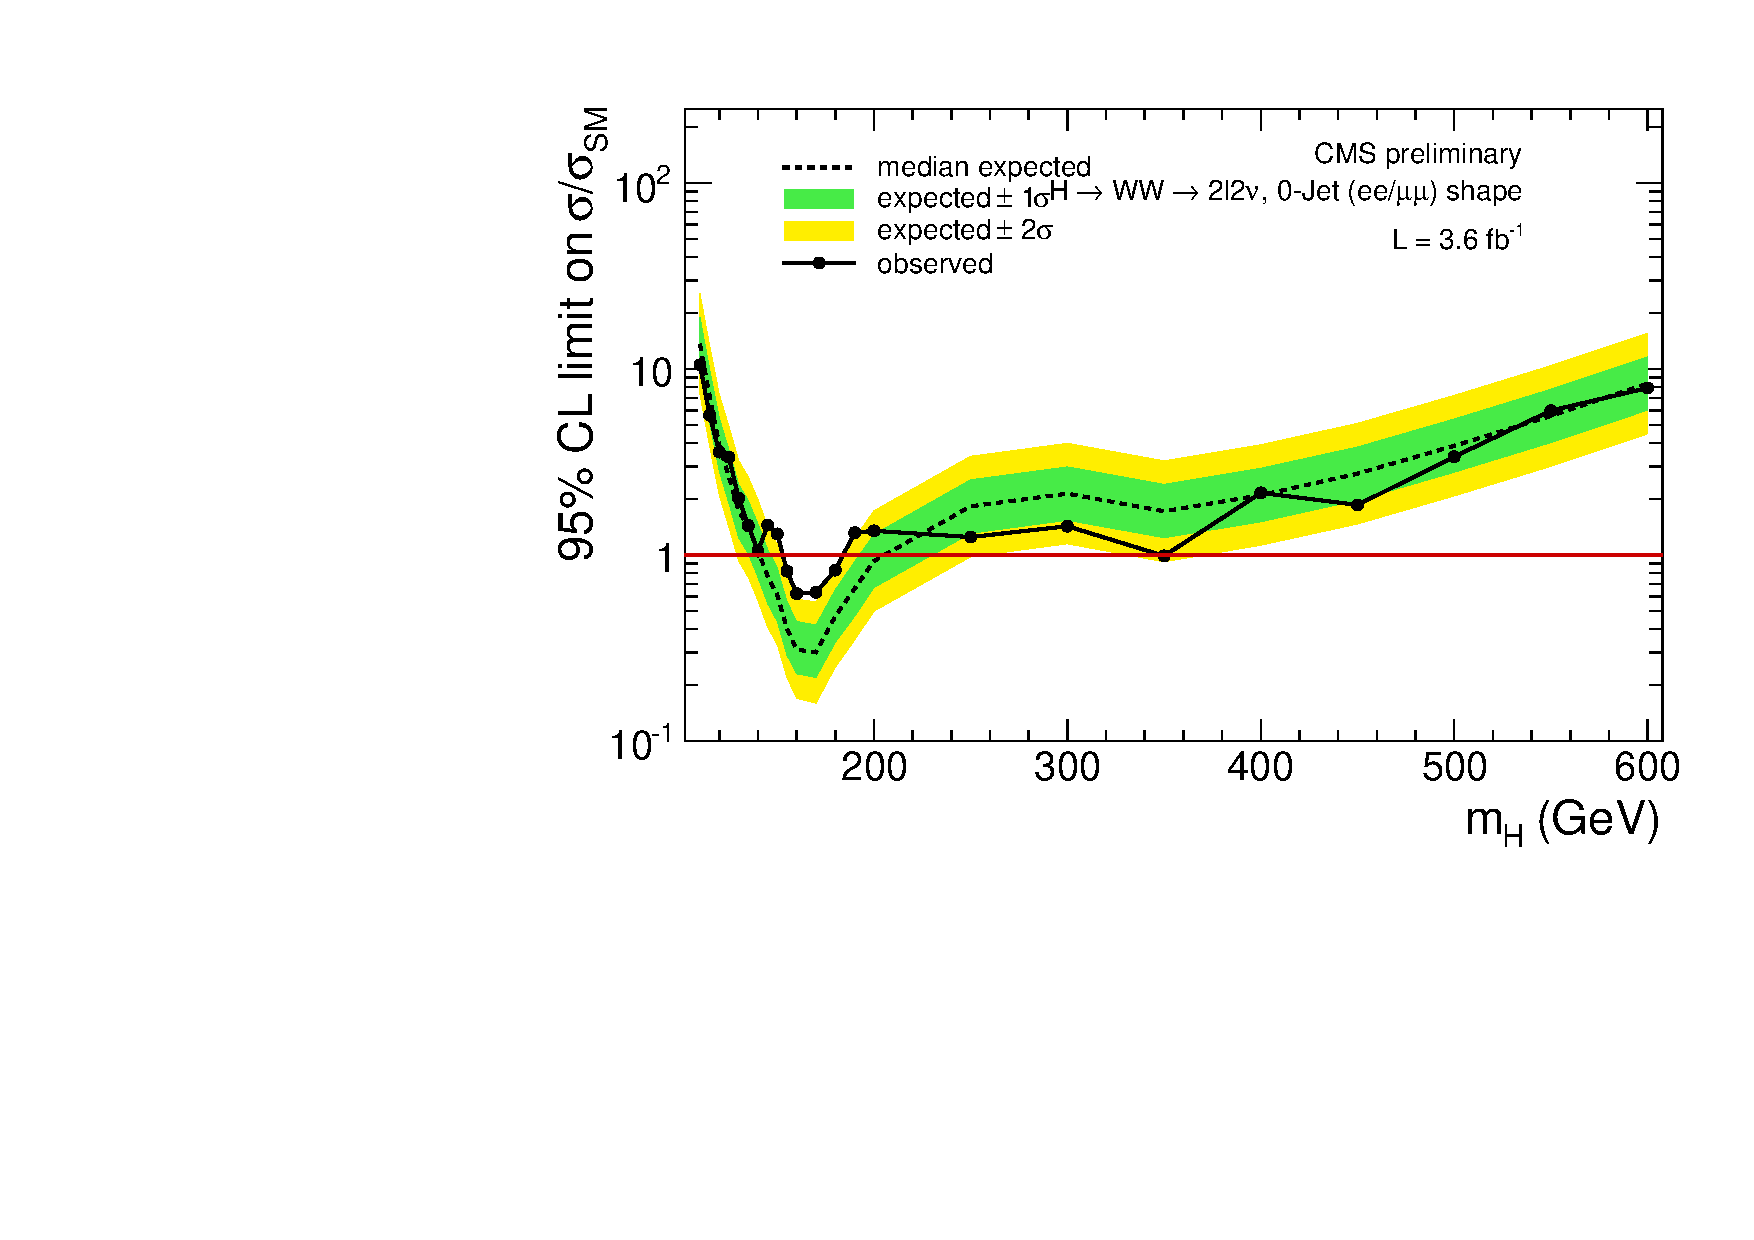
\includegraphics[width=.45\textwidth]{figures/limits_0jsf_shape-CLs-asymptotic_log.pdf}}
\centering
\subfigure[shape-based 0-Jet SF (zoom)]{
\centering
\label{subfig:0jsf_zoom_shape}
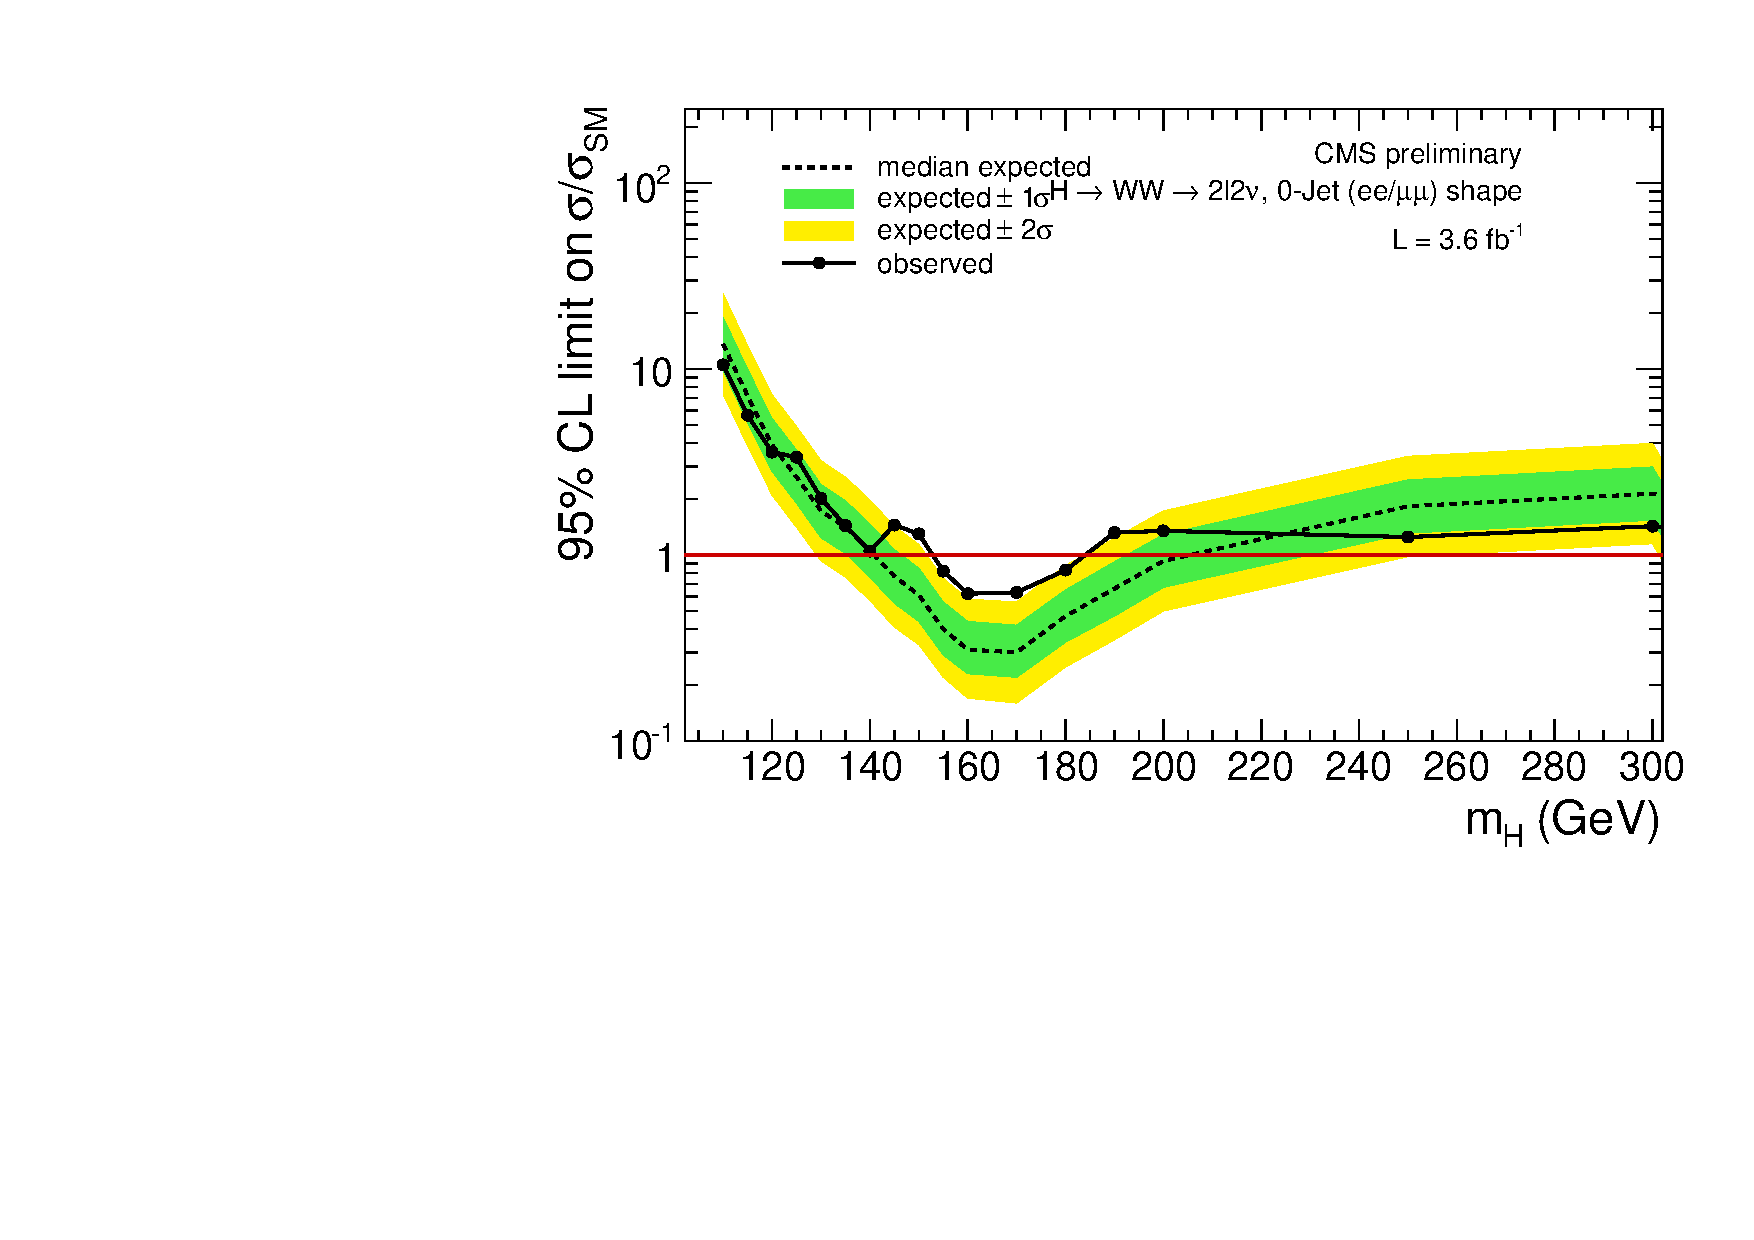
\includegraphics[width=.45\textwidth]{figures/limits_0jsf_shape-CLs-asymptotic_zoom_log.pdf}} \\
\label{fig:uls_shape_0j}
\caption{The expected and observed limits for the Shape-based analysis for 3.5/fb in the {\bf 0-Jet bin} 
using the {\bf CLs-asymptotic} approach. }
\end{figure}
%%%%%%%%%%%%%%%%%%%%%%%%%%%%%%


%%%%%%%%%%%%%%%%%%%%%%%%%%%%%%
\begin{figure}[!hbtp]
\centering
\subfigure[shape-based 1-Jet OF]{
\centering
\label{subfig:1jof_shape}
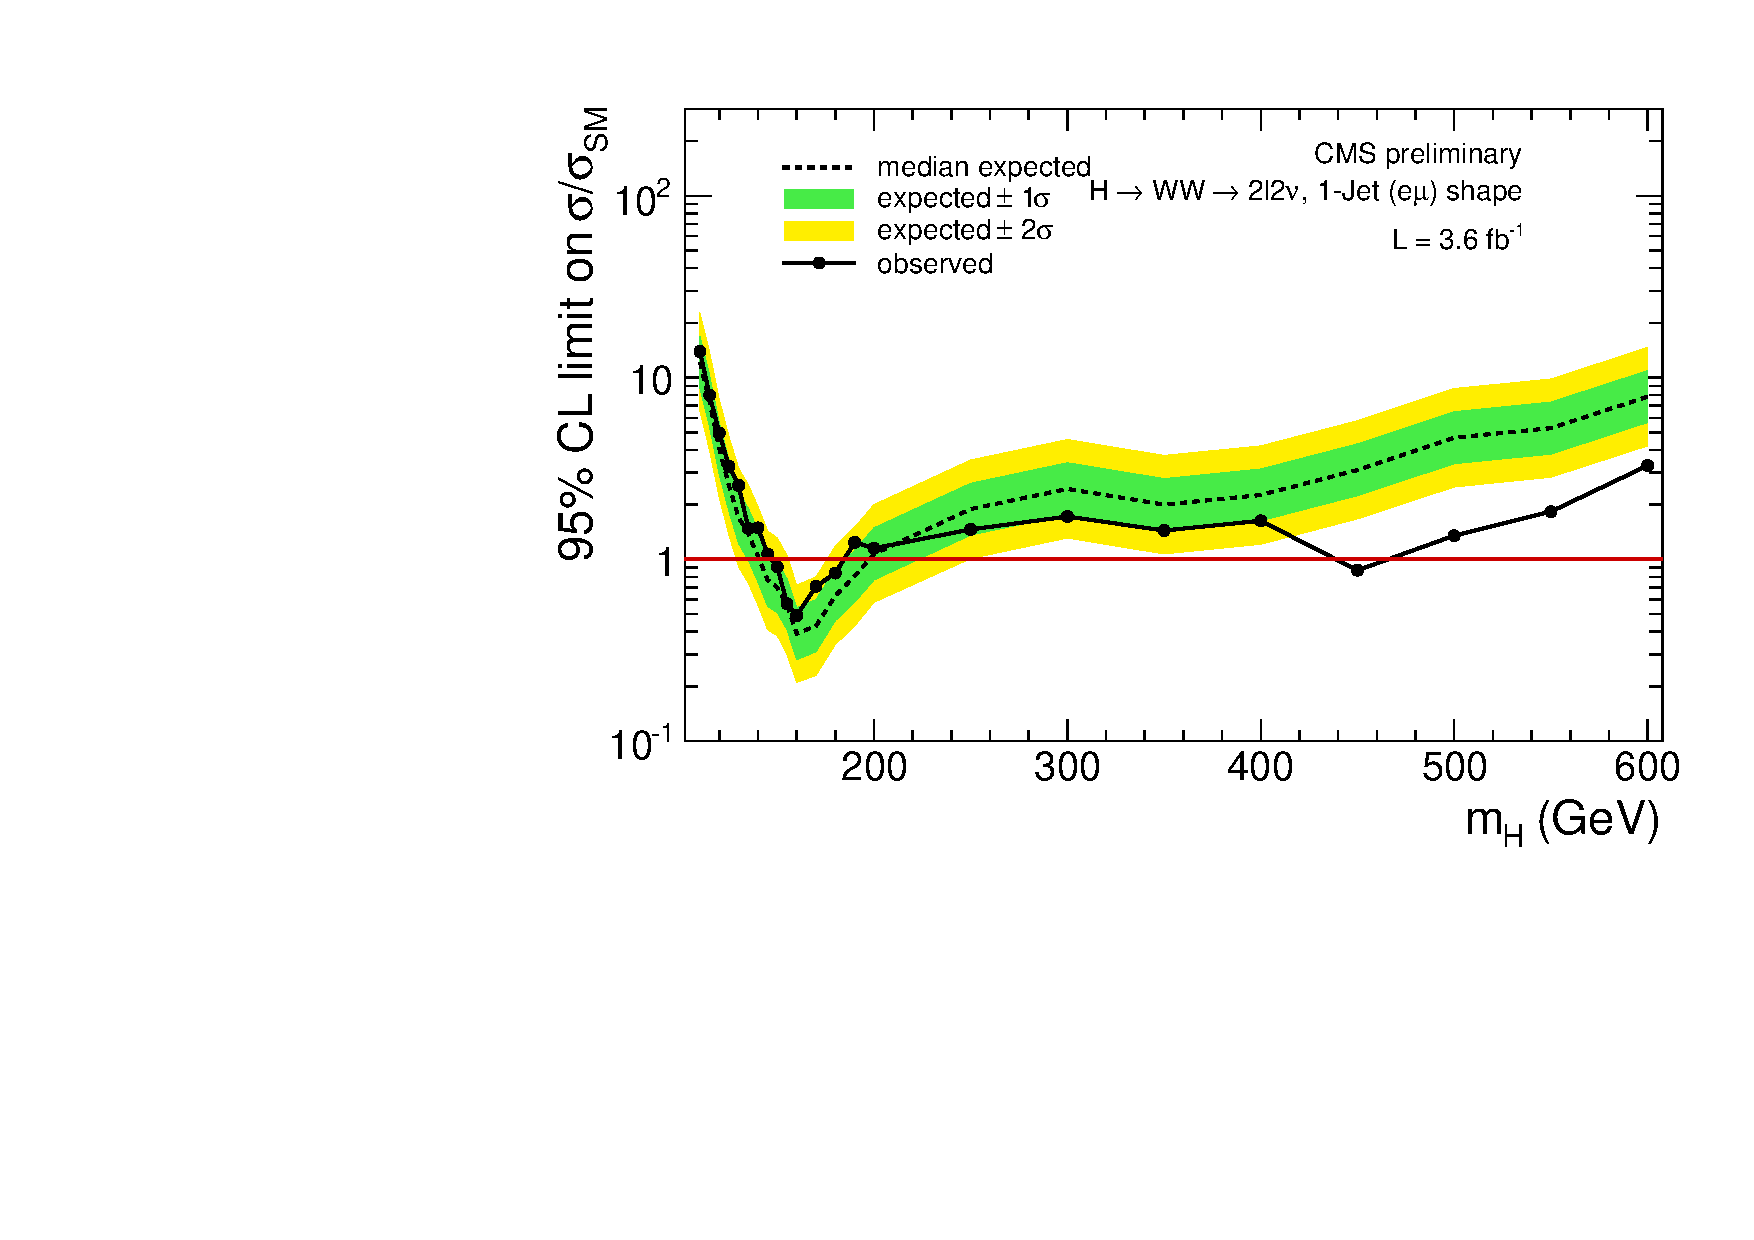
\includegraphics[width=.45\textwidth]{figures/limits_1jof_shape-CLs-asymptotic_log.pdf}}
\centering
\subfigure[shape-based 1-Jet OF (zoom)]{
\centering
\label{subfig:1jof_zoom_shape}
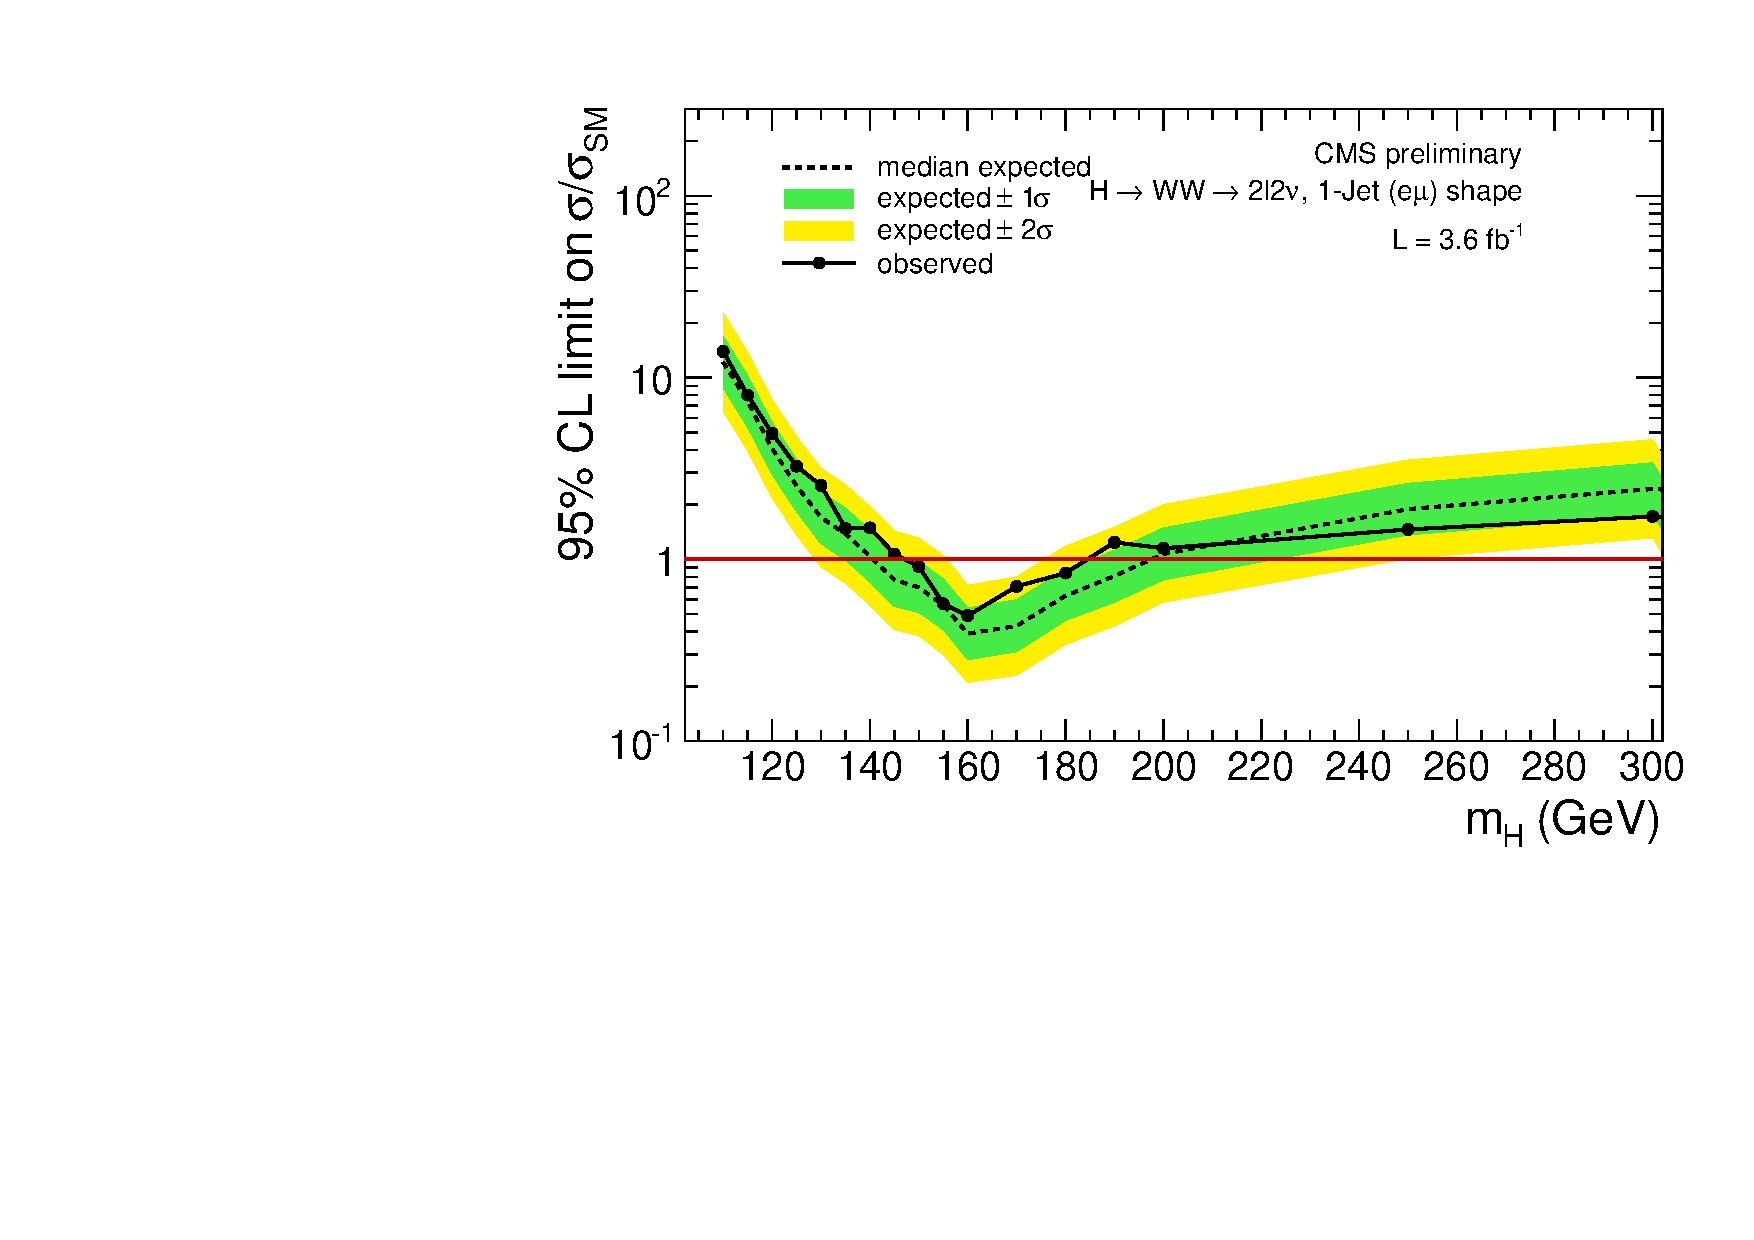
\includegraphics[width=.45\textwidth]{figures/limits_1jof_shape-CLs-asymptotic_zoom_log.pdf}} \\
\subfigure[shape-based 1-Jet SF]{
\centering
\label{subfig:1jsf_shape}
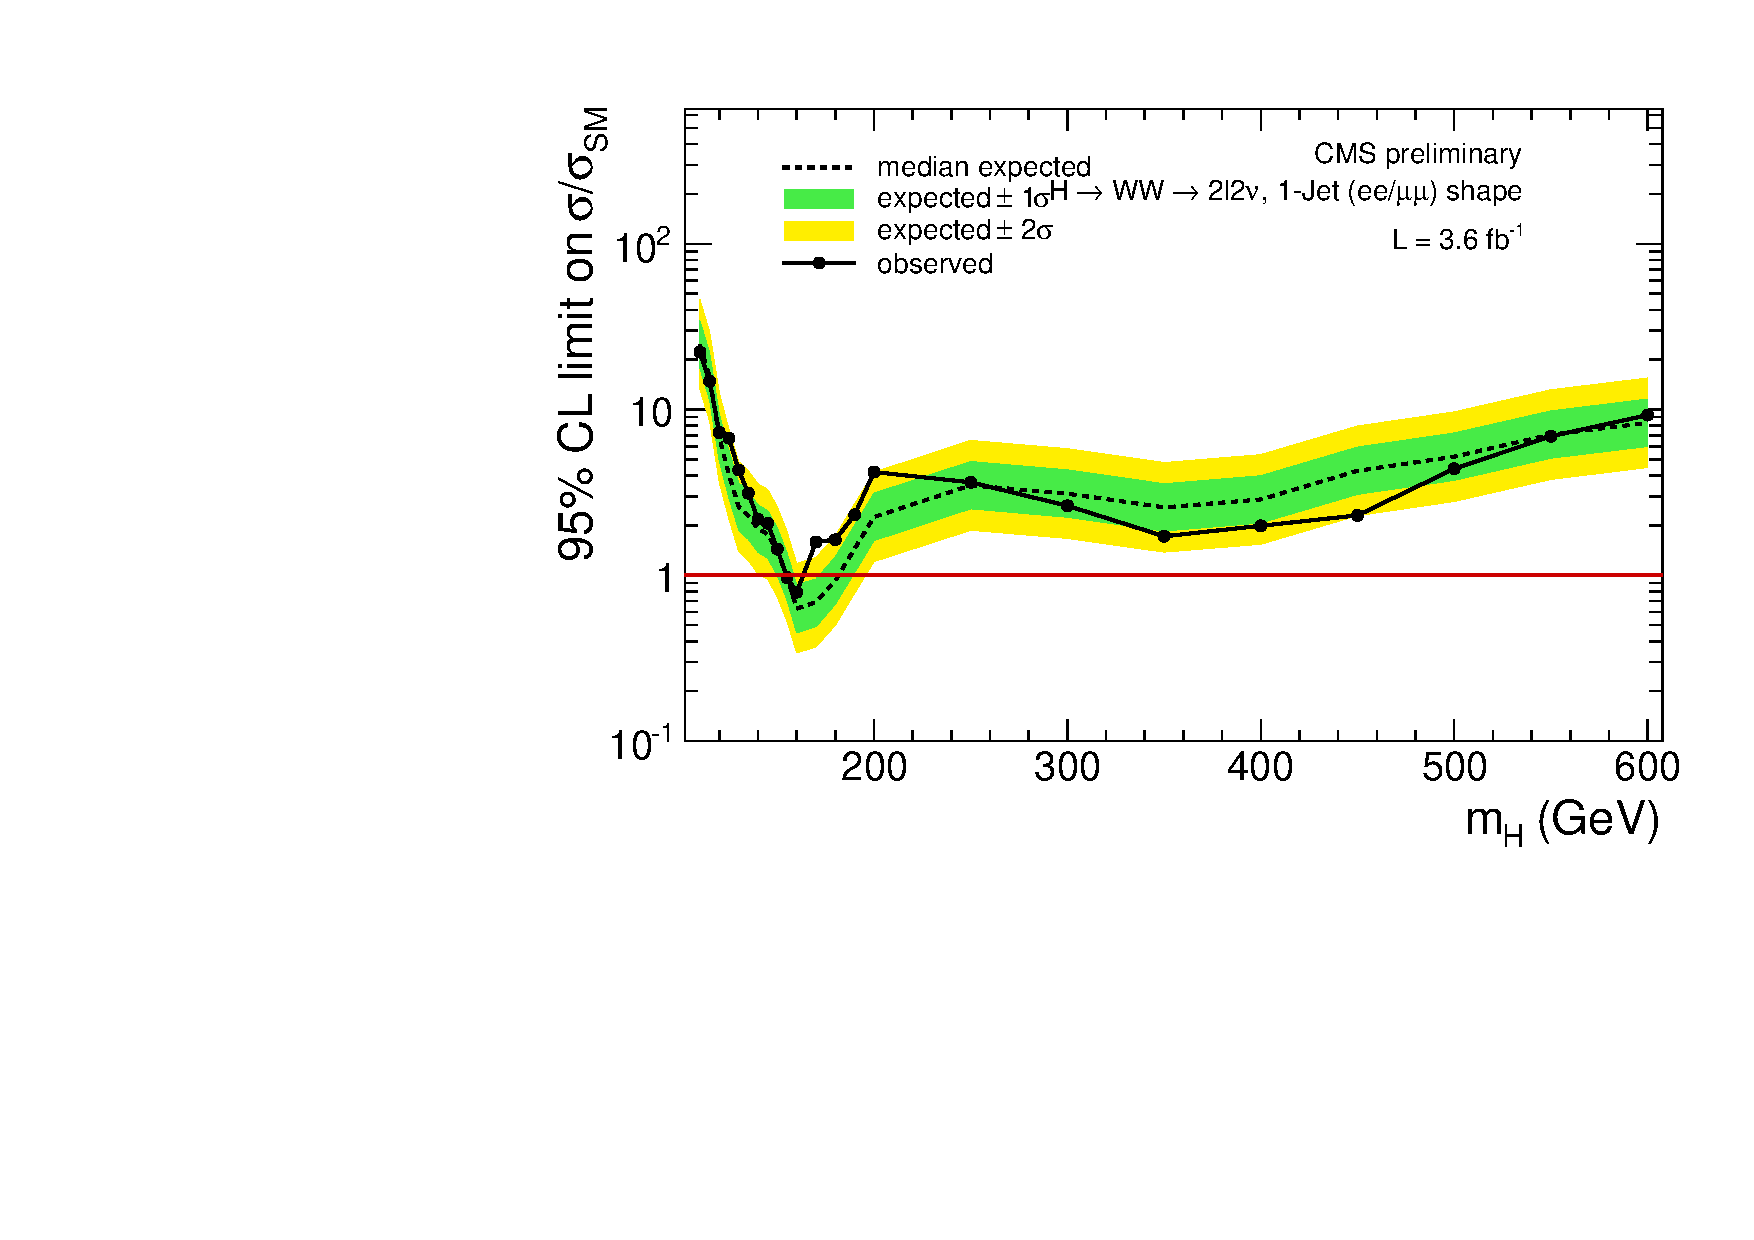
\includegraphics[width=.45\textwidth]{figures/limits_1jsf_shape-CLs-asymptotic_log.pdf}}
\centering
\subfigure[shape-based 1-Jet SF (zoom)]{
\centering
\label{subfig:1jsf_zoom_shape}
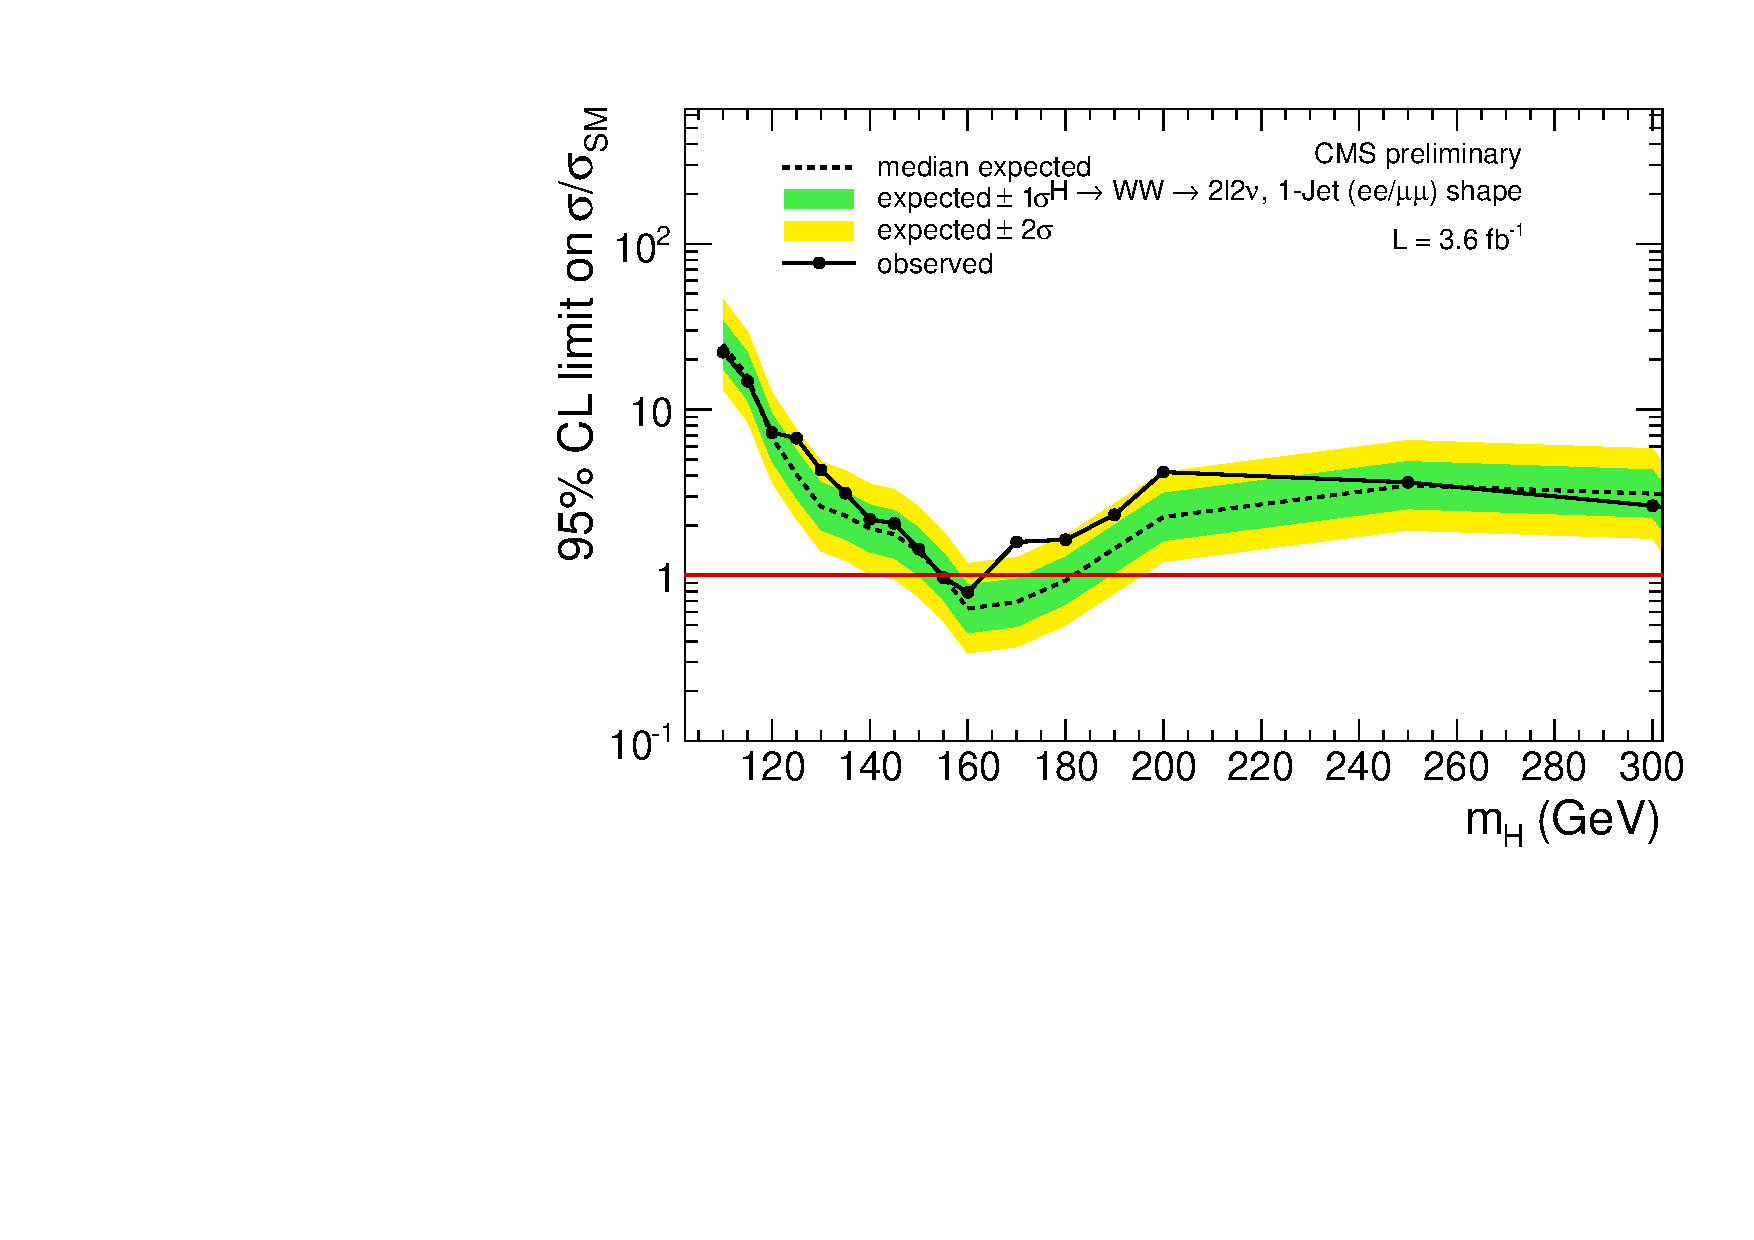
\includegraphics[width=.45\textwidth]{figures/limits_1jsf_shape-CLs-asymptotic_zoom_log.pdf}} \\
\label{fig:uls_shape_1j}
\caption{The expected and observed limits for the Shape-based analysis for 3.5/fb in the {\bf 1-Jet bin} 
using the {\bf CLs-asymptotic} approach. }
\end{figure}
%%%%%%%%%%%%%%%%%%%%%%%%%%%%%%

%%%%%%%%%%%%%%%%%%%%%%%%%%%%%%
\begin{table}[hbp!]
\begin{center}
\begin{tabular}{c c c c c}
\hline
\vspace{-3mm} && \\
 Higgs Mass & Observed  & Median expected & Expected range for 68\% & Expected range for 95\%   \\
\vspace{-3mm} && \\
\hline
110 & 11.5 & 8.1 & [5.8, 11.2] & [4.3, 15.1] \\
115 & 8.0 & 4.3 & [3.1, 6.0] & [2.3, 8.0] \\
120 & 5.0 & 2.5 & [1.8, 3.5] & [1.4, 4.7] \\
125 & 2.9 & 1.6 & [1.2, 2.3] & [0.9, 3.0] \\
130 & 1.6 & 1.2 & [0.8, 1.6] & [0.6, 2.2] \\
135 & 1.5 & 0.9 & [0.6, 1.2] & [0.5, 1.6] \\
140 & 1.4 & 0.7 & [0.5, 1.0] & [0.4, 1.3] \\
145 & 1.1 & 0.5 & [0.4, 0.8] & [0.3, 1.0] \\
150 & 1.0 & 0.5 & [0.3, 0.7] & [0.3, 0.9] \\
155 & 0.5 & 0.3 & [0.2, 0.5] & [0.2, 0.6] \\
160 & 0.4 & 0.3 & [0.2, 0.4] & [0.1, 0.5] \\
170 & 0.4 & 0.3 & [0.2, 0.4] & [0.2, 0.6] \\
180 & 0.4 & 0.4 & [0.3, 0.5] & [0.2, 0.7] \\
190 & 0.6 & 0.6 & [0.4, 0.8] & [0.3, 1.1] \\
200 & 1.0 & 0.8 & [0.6, 1.1] & [0.4, 1.4] \\
250 & 2.0 & 1.4 & [1.0, 1.9] & [0.7, 2.5] \\
300 & 2.9 & 1.7 & [1.2, 2.4] & [0.9, 3.2] \\
350 & 1.5 & 1.6 & [1.2, 2.2] & [0.9, 3.0] \\
400 & 1.3 & 1.8 & [1.3, 2.5] & [1.0, 3.4] \\
450 & 1.8 & 2.4 & [1.8, 3.4] & [1.3, 4.5] \\
500 & 2.4 & 3.3 & [2.4, 4.6] & [1.8, 6.2] \\
550 & 5.1 & 4.6 & [3.3, 6.4] & [2.5, 8.6] \\
600 & 5.8 & 6.5 & [4.7, 9.1] & [3.5, 12.2] \\
\hline
\end{tabular}
\caption{Expected and observed upper limits for SM Higgs using the
  {\bf Shape-based} analysis in the {\bf $e\mu$ OF 0-Jet bin} with \intlumiEightTeV\ of data.}
\label{tab:bdtbase_uls_0jof}
\end{center}
\end{table}
%%%%%%%%%%%%%%%%%%%%%%%%%%%%%%

%%%%%%%%%%%%%%%%%%%%%%%%%%%%%%
\begin{table}[hbp!]
\begin{center}
\begin{tabular}{c c c c c}
\hline
\vspace{-3mm} && \\
 Higgs Mass & Observed  & Median expected & Expected range for 68\% & Expected range for 95\%   \\
\vspace{-3mm} && \\
\hline
110 & 10.5 & 13.6 & [9.8, 19.0] & [7.3, 25.4] \\
115 & 5.7 & 7.2 & [5.2, 10.0] & [3.9, 13.4] \\
120 & 3.6 & 3.9 & [2.8, 5.4] & [2.1, 7.3] \\
125 & 3.4 & 2.6 & [1.9, 3.7] & [1.4, 4.9] \\
130 & 2.0 & 1.7 & [1.2, 2.4] & [0.9, 3.2] \\
135 & 1.4 & 1.4 & [1.0, 2.0] & [0.8, 2.6] \\
140 & 1.0 & 1.1 & [0.8, 1.5] & [0.6, 2.0] \\
145 & 1.4 & 0.8 & [0.6, 1.1] & [0.4, 1.4] \\
150 & 1.3 & 0.6 & [0.4, 0.8] & [0.3, 1.1] \\
155 & 0.8 & 0.4 & [0.3, 0.6] & [0.2, 0.7] \\
160 & 0.6 & 0.3 & [0.2, 0.4] & [0.2, 0.6] \\
170 & 0.6 & 0.3 & [0.2, 0.4] & [0.2, 0.6] \\
180 & 0.8 & 0.5 & [0.3, 0.7] & [0.3, 0.9] \\
190 & 1.3 & 0.7 & [0.5, 0.9] & [0.4, 1.2] \\
200 & 1.3 & 0.9 & [0.7, 1.3] & [0.5, 1.7] \\
250 & 1.2 & 1.8 & [1.3, 2.5] & [1.0, 3.4] \\
300 & 1.4 & 2.1 & [1.5, 3.0] & [1.1, 4.0] \\
350 & 1.0 & 1.7 & [1.2, 2.4] & [0.9, 3.2] \\
400 & 2.2 & 2.1 & [1.5, 2.9] & [1.1, 3.9] \\
450 & 1.9 & 2.7 & [2.0, 3.8] & [1.5, 5.1] \\
500 & 3.4 & 3.9 & [2.8, 5.4] & [2.1, 7.2] \\
550 & 6.0 & 5.6 & [4.0, 7.8] & [3.0, 10.4] \\
600 & 7.9 & 8.4 & [6.0, 11.6] & [4.5, 15.6] \\
\hline
\end{tabular}
\caption{Expected and observed upper limits for SM Higgs using the
  {\bf Shape-based} analysis in the {\bf $ee/\mu\mu$ SF 0-Jet bin} with \intlumiEightTeV\ of data.}
\label{tab:bdtbase_uls_0jsf}
\end{center}
\end{table}
%%%%%%%%%%%%%%%%%%%%%%%%%%%%%%
%%%%%%%%%%%%%%%%%%%%%%%%%%%%%%
\begin{table}[hbp!]
\begin{center}
\begin{tabular}{c c c c c}
\hline
\vspace{-3mm} && \\
 Higgs Mass & Observed  & Median expected & Expected range for 68\% & Expected range for 95\%   \\
\vspace{-3mm} && \\
\hline
110 & 13.9 & 12.2 & [8.8, 16.9] & [6.5, 22.7] \\
115 & 8.0 & 7.4 & [5.3, 10.3] & [4.0, 13.8] \\
120 & 4.9 & 4.1 & [2.9, 5.7] & [2.2, 7.6] \\
125 & 3.3 & 2.5 & [1.8, 3.5] & [1.4, 4.7] \\
130 & 2.6 & 1.7 & [1.2, 2.4] & [0.9, 3.2] \\
135 & 1.5 & 1.4 & [1.0, 1.9] & [0.7, 2.6] \\
140 & 1.5 & 1.0 & [0.8, 1.5] & [0.6, 1.9] \\
145 & 1.1 & 0.8 & [0.6, 1.1] & [0.4, 1.4] \\
150 & 0.9 & 0.7 & [0.5, 1.0] & [0.4, 1.3] \\
155 & 0.6 & 0.6 & [0.4, 0.8] & [0.3, 1.1] \\
160 & 0.5 & 0.4 & [0.3, 0.5] & [0.2, 0.7] \\
170 & 0.7 & 0.4 & [0.3, 0.6] & [0.2, 0.8] \\
180 & 0.8 & 0.6 & [0.5, 0.9] & [0.3, 1.2] \\
190 & 1.2 & 0.8 & [0.6, 1.1] & [0.4, 1.5] \\
200 & 1.2 & 1.1 & [0.8, 1.5] & [0.6, 2.0] \\
250 & 1.5 & 1.9 & [1.4, 2.6] & [1.0, 3.5] \\
300 & 1.7 & 2.4 & [1.8, 3.4] & [1.3, 4.6] \\
350 & 1.4 & 2.0 & [1.4, 2.8] & [1.1, 3.7] \\
400 & 1.6 & 2.3 & [1.6, 3.1] & [1.2, 4.2] \\
450 & 0.9 & 3.1 & [2.2, 4.3] & [1.7, 5.8] \\
500 & 1.4 & 4.7 & [3.4, 6.5] & [2.5, 8.7] \\
550 & 1.8 & 5.3 & [3.8, 7.3] & [2.8, 9.8] \\
600 & 3.3 & 7.9 & [5.7, 10.9] & [4.2, 14.6] \\
\hline
\end{tabular}
\caption{Expected and observed upper limits for SM Higgs using the
  {\bf Shape-based} analysis in the {\bf $e\mu$ OF 1-Jet bin} with \intlumiEightTeV\ of data.}
\label{tab:bdtbase_uls_1jof}
\end{center}
\end{table}
%%%%%%%%%%%%%%%%%%%%%%%%%%%%%%

%%%%%%%%%%%%%%%%%%%%%%%%%%%%%%
\begin{table}[hbp!]
\begin{center}
\begin{tabular}{c c c c c}
\hline
\vspace{-3mm} && \\
 Higgs Mass & Observed  & Median expected & Expected range for 68\% & Expected range for 95\%   \\
\vspace{-3mm} && \\
\hline
110 & 22.2 & 24.6 & [17.7, 34.3] & [13.2, 46.0] \\
115 & 14.8 & 15.8 & [11.4, 22.0] & [8.5, 29.5] \\
120 & 7.3 & 6.8 & [4.9, 9.4] & [3.6, 12.6] \\
125 & 6.7 & 4.1 & [2.9, 5.6] & [2.2, 7.6] \\
130 & 4.3 & 2.6 & [1.9, 3.6] & [1.4, 4.9] \\
135 & 3.1 & 2.3 & [1.6, 3.2] & [1.2, 4.3] \\
140 & 2.2 & 1.9 & [1.4, 2.7] & [1.0, 3.6] \\
145 & 2.1 & 1.8 & [1.3, 2.5] & [0.9, 3.3] \\
150 & 1.4 & 1.4 & [1.0, 1.9] & [0.7, 2.6] \\
155 & 1.0 & 1.0 & [0.7, 1.4] & [0.5, 1.8] \\
160 & 0.8 & 0.6 & [0.5, 0.9] & [0.3, 1.2] \\
170 & 1.6 & 0.7 & [0.5, 1.0] & [0.4, 1.3] \\
180 & 1.6 & 0.9 & [0.7, 1.3] & [0.5, 1.7] \\
190 & 2.3 & 1.4 & [1.0, 2.0] & [0.8, 2.7] \\
200 & 4.2 & 2.2 & [1.6, 3.1] & [1.2, 4.2] \\
250 & 3.6 & 3.5 & [2.5, 4.9] & [1.9, 6.5] \\
300 & 2.6 & 3.1 & [2.2, 4.3] & [1.7, 5.8] \\
350 & 1.7 & 2.6 & [1.8, 3.6] & [1.4, 4.8] \\
400 & 2.0 & 2.9 & [2.1, 4.0] & [1.5, 5.4] \\
450 & 2.3 & 4.3 & [3.1, 5.9] & [2.3, 8.0] \\
500 & 4.4 & 5.2 & [3.7, 7.2] & [2.8, 9.7] \\
550 & 6.9 & 7.1 & [5.1, 9.8] & [3.8, 13.2] \\
600 & 9.3 & 8.3 & [6.0, 11.6] & [4.5, 15.5] \\
\hline
\end{tabular}
\caption{Expected and observed upper limits for SM Higgs using the
  {\bf Shape-based} analysis in the {\bf $ee/\mu\mu$ SF 1-Jet bin} with \intlumiEightTeV\ of data.}
\label{tab:bdtbase_uls_1jsf}
\end{center}
\end{table}
%%%%%%%%%%%%%%%%%%%%%%%%%%%%%%
\clearpage
